\documentclass[11pt,letterpaper]{article}
\usepackage[T1]{fontenc}
\usepackage[utf8]{inputenc}
\usepackage{lmodern,microtype}
\usepackage[margin=1in]{geometry}
\usepackage{amsmath,amssymb,amsthm,mathtools,bm}
\usepackage{booktabs,longtable,array,enumitem}
\usepackage{graphicx,xcolor}
\usepackage{fancyhdr}
\usepackage{xurl}
\usepackage{hyperref}
\definecolor{navy}{HTML}{15395B}
\definecolor{teal}{HTML}{087F8C}
\hypersetup{colorlinks=true,linkcolor=navy,citecolor=teal,urlcolor=teal,
  pdftitle={Active Normal Faces and Batched Geometric Descent for Unknot Recognition},
  pdfauthor={Research continuation for the ProveIt project}}
\usepackage[nameinlink,noabbrev]{cleveref}
\usepackage{listings}
\lstset{basicstyle=\ttfamily\small,breaklines=true,columns=fullflexible,
  frame=single,rulecolor=\color{black!15},backgroundcolor=\color{black!2},
  showstringspaces=false}
\newtheorem{theorem}{Theorem}[section]
\newtheorem{lemma}[theorem]{Lemma}
\newtheorem{proposition}[theorem]{Proposition}
\newtheorem{corollary}[theorem]{Corollary}
\theoremstyle{definition}
\newtheorem{definition}[theorem]{Definition}
\newtheorem{example}[theorem]{Example}
\theoremstyle{remark}
\newtheorem{remark}[theorem]{Remark}
\newcommand{\R}{\mathbb R}
\newcommand{\Q}{\mathbb Q}
\newcommand{\Z}{\mathbb Z}
\newcommand{\supp}{\operatorname{supp}}
\newcommand{\rank}{\operatorname{rank}}
\newcommand{\spanof}{\operatorname{span}}
\newcommand{\peel}{\operatorname{peel}}
\newcommand{\poly}{\operatorname{poly}}
\newcommand{\M}{\mathsf M}
\newcommand{\basecommit}{\texttt{66098968e88bba797143ac1bf7ad0ac4c5f697df}}
\setlength{\headheight}{14pt}
\pagestyle{fancy}
\fancyhf{}
\fancyhead[L]{\small\color{navy}Active faces and geometric descent}
\fancyhead[R]{\small ProveIt research}
\fancyfoot[C]{\thepage}
\setlist{itemsep=3pt,topsep=5pt}
\setlength{\emergencystretch}{2em}

\begin{document}
\begin{titlepage}
\color{navy}
\noindent\textsf{PROVEIT / TOPOLOGY / UNKNOT RECOGNITION}\par
\vspace{1.0in}
\noindent{\Huge\bfseries Active Normal Faces\par}
\vspace{0.15in}
\noindent{\Huge\bfseries and Batched\par}
\vspace{0.15in}
\noindent{\Huge\bfseries Geometric Descent\par}
\vspace{0.35in}
\noindent{\Large Certified improvements for unknot recognition}\par
\vspace{0.5in}
\noindent{\large Research continuation for Vladimir Reshetnikov}\par
\vspace{0.15in}
\noindent 9 October 2026\par
\vfill
\color{black}
\noindent\textbf{Scope.} Exact support certificates, a structural obstruction to
root-level propagation, simultaneous Pachner reductions, and dynamic
vertex-link scoring. The complete recognizer's general quasipolynomial
complexity remains unproved.\par
\vspace{0.25in}
\noindent\textbf{Reproducible baseline.}\par
\noindent\basecommit\par
\smallskip
\noindent\url{https://github.com/VladimirReshetnikov/ProveIt}
\end{titlepage}

\begin{abstract}
We develop and implement certified improvements at two interfaces of the
ProveIt unknot-recognition programme. The principal geometric result is an
exact polynomial reduction of optimal vertex-link-peeled Euler scoring,
over every subbatch of a fixed tetrahedron-disjoint family of coherent
$3$--$2$ Pachner moves, to maximum-weight matching. A minimum-omission
optimum omits at most one move per relevant interior vertex. The maintained
pulling construction has exactly two interior vertices, so its optimum
omits at most two moves and its matching stage has a linear arithmetic-time
selector.
The conflict graph of all distinct legal central edges has degree at most
nine; consequently a packed optimum retains at least
$\max\{0,\lceil M/10\rceil-2\}$ of $M$ current candidates. We also prove
relative-boundary commutation, implement one simultaneous certificate, and
maintain exact peeling minima with deterministic balanced trees. A genuine
32-tetrahedron solid-torus example shows why adding singleton peeled scores
would be incorrect.

On the linear-programming side, a primal--dual pair certifies the entire
active support of a rational nonnegative matching cone. A homogeneous lift
produces that pair or an ordinary small negative certificate. An adaptive
quadrilateral search has at most $2^{\rho+1}-1$ nodes in terms of an intrinsic
active ambiguity rank $\rho$. However, explicit local normal-coordinate
directions prove $\rho\ge t-v$ at unrestricted anchored roots, and
$\rho\ge16\max\{1,n\}-2$ on the maintained $n$-crossing pulling source.
This is a structural obstruction to obtaining a universal polylogarithmic
bound from active support alone.

The additive implementation includes independent consumers, exact replay
fixtures, paired timing data, and a pinned integration patch. Four
64-move workloads show approximately $117$--$123$-fold producer improvements
over literal sequential replay, while the enlarged support LP regresses
against small unary probes. These are subroutine results. We identify the
remaining witness-coverage, transition-count, anchor, and bit-complexity
theorems required for a complete quasipolynomial recognizer, and propose a
concrete research programme to address them.
\end{abstract}


\tableofcontents
\clearpage
\section{Research question and precise contribution}

The computational objective is a complete unknot recognizer with a
quasipolynomial worst-case bound in the crossing number. The maintained
ProveIt implementation combines exact filters, group-theoretic methods,
normal-surface certificates, and a complete fallback. Many local operations
are now substantially faster than their first implementations. The central
research issue is whether the number and encoded size of the states visited
can be bounded without expanding exponentially large surfaces or returning
to an exhaustive search over all normal-coordinate sectors.

This continuation works on two interfaces where the existing research
packages leave concrete opportunities. In the normal-coordinate search,
syntactically allowed quadrilateral types need not be geometrically
possible. A certificate of the entire active support makes it possible to
remove these spurious choices in one operation and define the remaining
ambiguity intrinsically. In geometric descent, many currently legal
Pachner reductions have disjoint tetrahedral supports. They can be verified
and applied together, avoiding repeated emission and validation of almost
identical triangulations. Vertex-link peeling then requires careful
collective scoring: disjoint tetrahedral supports can still share a global
vertex, so their peeled scores need not add.

\subsection{What is established here}

The mathematical results fall into five groups.
\begin{enumerate}
\item A primal--dual description of the maximal active support of a
nonnegative homogeneous matching cone. A single aggregate dual witness
certifies every universally zero coordinate. Combining this with a
positive objective gives a complete support certificate, independently
checkable without rerunning the search procedure. The underlying
polyhedral principle is classical strict complementarity; the contribution
is its concrete certificate use at this repository interface.
\item An ambiguity parameter for restricted quadrilateral search, together
with a finite search-tree bound, and a negative result: on an unrestricted
one-vertex anchored root that has a positive-Euler witness, the ambiguity
rank is at least $t-1$. More generally it is at least $t-v(T)$,
and at least $16\max\{1,n\}-2$ on the maintained pulling source. The obstruction is explicit and comes from local
directions invisible to all face-arc equations.
\item A simultaneous relative-boundary replacement theorem for disjoint
$3$--$2$ regions. The conflict graph of distinct legal degree-three central
edges has maximum degree at most nine. A greedy maximal batch therefore
contains at least a tenth of the current candidates. The cocycle transport
and unpeeled cell changes commute and add.
\item A deterministic data structure that maintains vertex-link minima
under repeated local replacements. Cached thirteen-record prefixes give
constant-operation hypothetical singleton scoring, while balanced-tree
updates replenish these prefixes after commits. Collective scoring accounts
for shared vertices. A realized solid-torus example proves that singleton
peeled gains cannot simply be added.
\item An exact maximum-weight-matching reduction for the best peeled-Euler
subbatch of any fixed disjoint family. A minimum-omission optimum omits
at most one move per relevant interior vertex. On the maintained pulling
source, which has exactly two interior poles, a linear arithmetic-time
selector omits at most two moves. Thus the packed optimum retains at least
$\max\{0,\lceil M/10\rceil-2\}$ current candidates.
\end{enumerate}

All statements are scoped to their actual inputs. A positive-Euler relaxed
matching vector may violate the quadrilateral constraints. A legal Pachner
move preserves the ambient manifold, but coherent surfaces transported
through it can change topology. A positive total Euler characteristic is
therefore not an unknot certificate. The supplied code retains the
repository's independently verified component-disc query as the relevant
terminal geometric test.

\subsection{Position relative to the latest incoming work}

The source revision inspected is \basecommit. Its \texttt{fast/} and
\texttt{synthesis/} files used here were verified against their Git blob
identities. The three relevant archives in \texttt{docs/incoming/} were
also verified byte-for-byte against the repository's recorded blobs:
the dual-certificates report, the support-sensitive-certificates report,
and the geometric-transport report, all dated 9 October 2026
\cite{priorDual,priorSupport,priorTransport}. They are prior work, not new
deliverables of this continuation.

The dual report introduced independently replayable LP objective
certificates and forced-type propagation. The support report sharpened
component-incidence bounds and primitive ray certification. The transport
report established the exact five-height Pachner score, coherent cocycle
transport, and the thirteen-record lemma for a \emph{fixed} scoring pass.
It explicitly left that last lemma unimplemented and warned that a short
prefix must be replenished after repeated deletions. The present dynamic
construction supplies that missing maintenance mechanism and connects it
to simultaneous geometric replacements.

The package contains a pinned supporting snapshot, a small overlay for
the new modules, an integration patch, exact proof fixtures, retained
measurements, and reproduction scripts. It is prepared for review and
integration; no remote repository modification is part of this task.

\subsection{The literature does not remove the global gap}

Lackenby's technical announcement describes a hierarchy strategy with a
quasipolynomial running-time target \cite{LackenbyTalk}. The particular
Oxford handout gives $2^{O((\log n)^3)}$, which is
$n^{O((\log n)^2)}$. This should not be silently replaced by the sharper
$n^{O(\log n)}$ expression sometimes quoted in public descriptions.
Both are quasipolynomial, but the exponent matters in a rigorous cost
ledger.

The July 2026 preprint gives a substantial hierarchy-based recognition
algorithm and new certificate results \cite{Lackenby2026}. Its discussion
of running time explicitly leaves algorithmic precision and speed-up
for further work. Proposition~10.2 bounds the length of a partial
hierarchy by a linear function of quadrilateral handle complexity; it
does not establish the missing polylogarithmic effective-depth statement
for the code developed here.

The normal-coordinate part also has important established precedents.
Burton--Ozlen's tree traversal uses LP feasibility and greedy support
minimization to obtain a connected positive-Euler surface
\cite{BurtonOzlen}. Burton's admissible-face theory identifies compatibility
with the geometry of nonnegative normal cones \cite{BurtonFaces}. The new
support certificate must be understood against those results. We neither
claim that LP support reduction is new nor infer a polynomial recognition
algorithm from the polynomial solvability of a single LP.

\section{Geometric, algebraic, and encoding conventions}

\subsection{Finite triangulations and local identifications}

Let $T$ be a finite generalized triangulation with $t$ tetrahedra. Each
tetrahedron has four numbered vertices. A face is either unpaired or is
paired to another face by a permutation of the four local vertices.
The reciprocal pairing and its inverse are both recorded. Local corners,
edges, and faces are distinguished from global equivalence classes under
these identifications. In particular, several corners of a tetrahedron
can represent the same global vertex.

The implemented geometric validator requires a connected orientable
compact three-manifold with one torus boundary component. It checks
reciprocal pairings, orientation consistency, edge identifications,
vertex links, and the boundary's connectedness and Euler characteristic.
An interior vertex link is a sphere; a boundary vertex link is a disc.
These are the hypotheses under which the following normal-coordinate and
Pachner operations are used. Establishing that an arbitrary supplied
triangulation is the exterior of the user's knot is a separate provenance
obligation, supported by the repository's diagram-exterior routines.

\subsection{Normal coordinates}

Write a standard normal vector as
\[
 x=(a_{iv},q_{ij})\in\R_{\ge0}^{7t},
 \qquad 0\le i<t,\quad 0\le v<4,\quad 0\le j<3.
\]
Here $a_{iv}$ counts triangles cutting off vertex $v$ in tetrahedron $i$,
and $q_{ij}$ counts quadrilaterals of type $j$. Across each paired face,
the three normal-arc counts agree. These conditions form a sparse integer
linear system $Ax=0$. Each arc equation is a difference of two triangle
coordinates and two quadrilateral coordinates, with coincidences combined.
The additional quadrilateral condition requires at most one positive
$q_{ij}$ in each tetrahedron. It is this nonconvex condition that necessitates
sector choices or a different global method.

On the linear matching space the Euler characteristic is a rational
linear functional $c^Tx$. One may calculate it by assigning each global
edge-intersection count to a representative local edge and counting one
copy of each glued normal arc. For integral admissible vectors the result
is the integer Euler characteristic of the corresponding surface.
The linear formula remains algebraically defined on relaxed vectors
with incompatible quadrilaterals; those vectors do not necessarily
represent embedded surfaces.

The full integral vector can be very large in value but small in encoding.
Let $B$ bound the bit length of its coordinates or local height differences.
Algorithms here manipulate $O(t)$ binary integers, not one object per
normal disc. Any theoretical polynomial LP bound refers to the full
rational input bit length. The shipped exact simplex is an implementation
choice with explicit resource limits, and has no polynomial pivot bound.

\subsection{Anchors and vertex links}

For a global vertex $v$, let $C_v$ be its set of local corner records.
The normal vertex-link vector $L_v$ has one triangle at every corner in
$C_v$ and zero quadrilaterals. The maximal removable multiplicity is
\[
 m_v(x)=\min_{c\in C_v} a_c,
 \qquad
 \peel(x)=x-\sum_v m_v(x)L_v.
\]
The peeled vector is nonnegative, obeys the same matching equations,
and is admissible when $x$ is. Choosing one triangle coordinate at each
global vertex and setting it to zero gives an \emph{anchor face}. Every
peeled vector lies on some anchor face. A one-vertex triangulation has
at most $4t$ raw corner anchors, with additional contractions possible
as in the incoming dual report.

Peeling is distinct from division by the common divisor of quadrilateral
coordinates. The latter can be useful for component-count queries, but
it changes all coordinates and is not part of the local-update theorem.
For $\lambda_v=\chi(L_v)\in\{1,2\}$ and $d_v=|C_v|$,
\begin{equation}\label{eq:peel-identities}
 \chi(\peel(x))=\chi(x)-\sum_v\lambda_vm_v(x),
 \qquad
 P(\peel(x))=P(x)-\sum_vd_vm_v(x),
\end{equation}
where $P$ is the number of normal discs before gluing. These identities
also explain why vertices shared by disjoint local replacements can
couple their peeled scores.

\subsection{Integral cocycles and coherent fibres}

An integral cocycle can be represented in each tetrahedron by four
integer heights $h_{i0},\ldots,h_{i3}$. The signed height differences
agree on globally identified edges. Adding the same constant to all
four heights of one tetrahedron does not change those differences.
Sorting its four heights as $h_a\le h_b\le h_c\le h_d$ gives the
coherent normal vector with $h_b-h_a$ triangles at $a$,
$h_d-h_c$ triangles at $d$, and $h_c-h_b$ quadrilaterals separating
$\{a,b\}$ from $\{c,d\}$. Equal heights cause zero counts and require
no special perturbation.

The construction is the normal level set of the local affine height
functions, with unit-separated levels taken modulo integral shifts.
It is cooriented and its boundary and normal matching data agree under
face gluings. A transport operation preserves the integral cohomology
class but can split, join, or change components of this fibre. The
incoming transport package contains a verified example in which one
disc becomes a disc and two spheres \cite{priorTransport}. Thus component
analysis remains necessary after any geometric search policy.

\subsection{Cost model and certificate scope}

The comparison model counts arithmetic on integers separately from its
bit cost. An operation on a bounded number of $B$-bit heights takes
polynomial bit time in $B$; multiplication by a corner count introduces
$O(\log t)$ additional bits. We write $\M(b)$ for a chosen integer
multiplication cost and avoid treating a large integer as a machine word.
Combinatorial indices use $O(\log(t+2))$ bits.

Three kinds of output are deliberately distinct: an algebraic certificate
about a supplied matching system; a geometric certificate relating two
triangulations and transported cocycles; and a knot verdict tied to the
original diagram. The first two can accelerate the third but do not
replace its end-to-end proof requirements.

\section{Active normal cones: complete support proofs and a structural obstruction}
\label{sec:active-faces}

The previous continuation replaces some normal-ray enumeration queries by
exact positive-Euler linear programmes and certifies their negative answers
by Farkas multipliers.  It also identifies a difficulty with a strong
mandatory-type backdoor: a tetrahedron unused by a positive surface can
retain several allowed types, even when that surface is easy to find
\cite{priorDual}.  An immediate response is to distinguish an allowed
coordinate from one that is actually positive somewhere in the relaxed cone.
This section makes that distinction exact, implements its certificate, and
then proves a limitation of the resulting structural parameter.

The linear-programming ingredients are classical.  Strict complementarity
and maximal support belong to the Goldman--Tucker framework
\cite{GoldmanTucker}; coordinate-face traversal and normal-surface LP search
have substantial precedents \cite{BurtonFaces,BurtonOzlen}.  Our purpose is
to give a source-sized proof interface, an explicit homogeneous construction
compatible with the supplied exact solver, and a precise complexity bound
for the adaptive tree.  Familiar local matching identities then yield a
linear lower bound for its root parameter on genuine normal-coordinate
inputs, including the maintained diagram-exterior construction.

\subsection{One primal--dual pair identifies every active coordinate}

Let $A\in\Q^{m\times N}$ and $c\in\Q^N$.  Put
\begin{equation}\label{eq:active-cone-def}
 C=\{x\in\R^N:x\ge0,\ Ax=0\},\qquad
 S(C)=\{j:\text{some }z\in C\text{ has }z_j>0\}.
\end{equation}
The set $S(C)$ is the \emph{active support of the cone}; it need not equal the
support of a particular basic solution.  Write
$P_c=\{x\in C:c^Tx>0\}$.  If $P_c$ is nonempty, its active support is also
$S(C)$.  Indeed, if $p\in P_c$ and $z\in C$ has $z_j>0$, then
$p+\varepsilon z\in P_c$ for sufficiently small positive $\varepsilon$.
The objective of $z$ may be negative.  Activity on the positive-objective
part therefore cannot be inferred from the sign of an individual direction's
objective.

\begin{lemma}[Complete active-support alternative]\label{lem:active-pair}
Exactly one of the following alternatives holds:
\begin{enumerate}
\item There are rational vectors $x\in\Q^N$ and $y\in\Q^m$ satisfying
\begin{equation}\label{eq:active-primal-dual}
 Ax=0,\quad x\ge0,\quad c^Tx\ge1,\qquad
 s:=A^Ty\ge0,\quad x+s\ge\mathbf1.
\end{equation}
\item There is a rational vector $h\in\Q^m$ such that
\begin{equation}\label{eq:active-negative}
 A^Th\ge c.
\end{equation}
\end{enumerate}
In the first alternative, $x_j\ge1$ exactly when $j\in S(C)$, and
$s_j\ge1$ exactly when $j\notin S(C)$.
\end{lemma}

\begin{proof}
For a pair satisfying \eqref{eq:active-primal-dual},
\[
 x^Ts=x^TA^Ty=(Ax)^Ty=0.
\]
Both vectors are nonnegative.  Hence $x_js_j=0$ in every coordinate, while
$x_j+s_j\ge1$ ensures that exactly one of the two entries is at least one.
For any $z\in C$, the same calculation gives $z^Ts=0$.  Thus $s_j>0$
forces $z_j=0$ throughout $C$, whereas $x_j>0$ explicitly demonstrates
activity.  This proves the support assertion.

Suppose $P_c\ne\varnothing$.  For each $j\in S(C)$ choose a rational
$z^{(j)}\in C$ with $z^{(j)}_j>0$.  Rational witnesses exist because the
relevant linear systems are rational.  Their sum $z$ is positive on all of
$S(C)$.  Starting from a rational $p\in P_c$, choose a sufficiently small
positive rational $\varepsilon$ and then rescale $p+\varepsilon z$ to obtain
$x_j\ge1$ on $S(C)$ and $c^Tx\ge1$.

For every inactive coordinate $j$, the functional $e_j^Tz$ is nonpositive
on $C$; in fact it is identically zero.  The homogeneous Farkas alternative
gives a rational $y^{(j)}$ with $A^Ty^{(j)}\ge e_j$.  Let
$y=\sum_{j\notin S(C)}y^{(j)}$, with the empty sum interpreted as zero.
Its residual is nonnegative everywhere and at least one off $S(C)$.
Orthogonality with the constructed $x$ makes it zero on $S(C)$.  Thus
\eqref{eq:active-primal-dual} holds.

If $P_c=\varnothing$, homogeneous Farkas gives
\eqref{eq:active-negative}.  Conversely, pairing that inequality with any
nonnegative kernel vector gives $c^Tx\le h^TAx=0$, which excludes the first
alternative.
\end{proof}

The proof has a useful verification consequence.  The checker does not need
one infeasibility test per inactive coordinate, and it does not reproduce a
relative-interior algorithm.  It checks two matrix products, signs, and the
coordinatewise coverage inequality in \eqref{eq:active-primal-dual}.  One
multiplier exposes all inactive coordinates simultaneously; one positive
vector proves that no remaining coordinate has been silently omitted.

The claim is about the relaxed cone.  For example,
\[
 A=(1,-1),\qquad c=(1,1),\qquad C=\{(a,a):a\ge0\}
\]
has both coordinates active and positive objective away from zero.  If the
two coordinates are declared incompatible, it has no admissible positive
point.  A complete active-support vector can thus be a particularly
incompatible relaxation vector.

\subsection{A single homogeneous query with a small negative output}

The inherited solver accepts positive-objective queries over a nonnegative
homogeneous kernel.  We can use that interface directly.  Introduce
nonnegative variables
\[
 (x,y^+,y^-,s,u,v,\tau),
\]
where $x,s,u$ have $N$ entries, $y^+,y^-$ have $m$ entries, and $v,\tau$ are
scalars.  Impose
\begin{align}
 Ax&=0, &
 s-A^T(y^+-y^-)&=0,\label{eq:active-lift-a}\\
 x+s-u-\tau\mathbf1&=0, &
 c^Tx-v-\tau&=0.\label{eq:active-lift-b}
\end{align}
There are $3N+2m+2$ nonnegative variables and $m+2N+1$ equations.  The
objective is $\tau$.  A point with $\tau>0$, divided by $\tau$, yields
\eqref{eq:active-primal-dual} with $y=y^+-y^-$.  Conversely, split any
multiplier from that certificate into its positive and negative parts, set
$\tau=1$, and use the nonnegative surpluses for $u$ and $v$.  The lifted
positive query is therefore equivalent to $P_c\ne\varnothing$.

It is also possible to discard the large lifted dual after a negative
answer.  The following projection is useful because the consumer can remain
an ordinary homogeneous-Farkas checker on the original matrix.

\begin{proposition}[Projection of a lifted negative proof]
\label{prop:active-dual-projection}
Let $(\alpha,\beta,\gamma,\delta)$ be a negative Farkas multiplier for the
lifted positive-$\tau$ query, grouped according to the four displayed sets of
equations.  Then $\delta<0$, and $h=\alpha/(-\delta)$ satisfies
$A^Th\ge c$.
\end{proposition}

\begin{proof}
The lifted column inequalities are
\begin{align*}
 A^T\alpha+\gamma+\delta c&\ge0,& A\beta&=0,\\
 \beta+\gamma&\ge0,& \gamma&\le0,\\
 \delta&\le0,&-\mathbf1^T\gamma-\delta&\ge1.
\end{align*}
The equality $A\beta=0$ comes from the two oppositely signed columns for
each free dual variable.  If $\delta=0$, then
$\beta\ge-\gamma\ge0$.  Pairing the first inequality with $\beta$ gives
\[
 0\le\beta^T\gamma\le-\sum_j\gamma_j^2.
\]
Thus $\gamma=0$, which contradicts
$-\mathbf1^T\gamma-\delta\ge1$.  Hence $\delta<0$.  Finally,
\[
 A^T\alpha\ge-\gamma-\delta c\ge-\delta c,
\]
and division by $-\delta$ gives the required original-cone dual.
\end{proof}

The enlarged system has polynomial encoding length in the original rational
input.  Standard rational-LP algorithms consequently decide it in polynomial
bit complexity, with polynomial-bit primal or dual witnesses.  The executable
producer uses the exact Bland-simplex routine inherited from the previous
continuation \cite{priorDual}.  Its arithmetic is exact and its configured
pivot allowance is explicit; this implementation is not asserted to have a
polynomial worst-case pivot count.  The distinction is material: one large
degenerate LP can cost much more than several small support probes.  The
experiments section reports that tradeoff, including unfavorable outcomes.

\subsection{An intrinsic rank for the remaining incompatibilities}

Let $\mathcal G$ be a collection of coordinate conflict groups.  In normal
coordinates these are the three quadrilateral types in each tetrahedron.
A vector is admissible when each group contains at most one positive
coordinate.  The following definition also permits overlapping groups, since
the proof uses only their incompatibility disjunctions.

\begin{definition}[Active ambiguity rank]\label{def:active-ambiguity}
For $C$ as in \eqref{eq:active-cone-def}, let $V=\spanof(C)$ and put
\[
 J(C)=\bigcup_{\substack{G\in\mathcal G\\|G\cap S(C)|\ge2}}
             (G\cap S(C)).
\]
Define
\begin{equation}\label{eq:active-rho}
 \rho(C)=\dim\spanof\{e_j|_V:j\in J(C)\}.
\end{equation}
\end{definition}

This quantity depends on the cone and the conflict groups, not on the LP
solver's particular basic point.  Universally zero coordinates do not
contribute.  Neither do independent directions carried only by coordinates
outside every active conflict.

It is an exact linear-algebraic quantity once the active-support certificate
has been checked.  If $S=S(C)$, then
\begin{equation}\label{eq:active-dimension}
 V=\{z:Az=0,\ z_j=0\ (j\notin S)\},\qquad
 \dim V=|S|-\rank A_S.
\end{equation}
Indeed, a vector positive on $S$ has a relative neighborhood in
$\ker A_S$ that remains nonnegative, so the cone spans that entire kernel.
Writing $E_J$ for the indicated coordinate rows restricted to $S$ gives
\begin{equation}\label{eq:active-rho-rank}
 \rho(C)=\rank\begin{pmatrix}A_S\\E_J\end{pmatrix}-\rank A_S.
\end{equation}
Rank computation is useful for interpretation and complexity accounting; the
certificate checker does not need to trust a reported rank in order to accept
a positive witness or a negative search tree.

\begin{theorem}[Binary active-face search]\label{thm:active-tree}
Suppose $C$ contains a point of positive objective.  At each nonterminal
positive node, compute complete active support and choose any incompatible
active pair $i,j$.  Recurse on
\[
 C\cap\{x_i=0\}\qquad\text{and}\qquad C\cap\{x_j=0\}.
\]
Terminate at a nonpositive cone or at a positive cone whose active support is
compatible.  This decides admissible positive-objective existence.  Its
complete binary tree has at most $2^{\rho(C)+1}-1$ nodes.  With polynomial
rational LP, its bit cost and certificate length are
$2^{\rho(C)}\poly(L)$, where $L$ is the original encoded input length.
\end{theorem}

\begin{proof}
Every admissible vector satisfies $x_i=0$ or $x_j=0$, so the two children cover
all admissible possibilities.  Their overlap is harmless.  A coordinate
deleted using an active-support dual is zero on the entire current cone;
such a deletion preserves every admissible candidate.  A negative dual
excludes positive objective.  At a compatible positive leaf, the active
primal vector is itself admissible.  These observations prove correctness.

For the bound, let $C'$ be a child whose positive-objective part is nonempty,
and put $V'=\spanof(C')$.  Coordinate restriction cannot create new active
coordinates, so $J(C')\subseteq J(C)$.  Let
\[
 W=\spanof\{e_k|_V:k\in J(C)\}.
\]
In the child $x_i=0$, restriction from $V$ to $V'$ kills $e_i|_V$.  That
functional is nonzero because $i$ was active, and it belongs to $W$ because
$i$ was part of an active conflict.  The restriction map on $W$ therefore
has nontrivial kernel.  Its image has dimension at most $\rho(C)-1$, and
the defining functionals for $\rho(C')$ lie in that image.  Consequently
\[
 \rho(C')\le\rho(C)-1.
\]
The same argument applies to the other child.

If $\rho=0$, there is no active incompatible pair: any active coordinate in
such a pair would be a nonzero defining functional.  Hence every positive
branching node has rank at least one.  Along a path, ranks decrease at each
edge whose child remains positive.  A final negative leaf can occur after
the last rank-one branching node, so the full path still contains at most
$\rho(C)$ branches.  Binary tree counting yields the stated node bound.
Every query and arithmetic witness has polynomial encoded size, and a
negative tree retains both children at each split, giving the time and
certificate estimates.
\end{proof}

The proof makes no assumption that the selected coordinate-zero face drops
dimension by exactly one.  A child may lose several coordinates at once,
which only improves the bound.  It also permits additional early terminal
rules.  In particular, a small ordinary LP may first return a negative dual
or an already admissible basic vector.  Stopping in either case shortens the
tree.  The implementation uses this precheck by default and invokes the
larger active-support LP only for an incompatible positive relaxation.

\subsection{Normal anchors and the precise scope of a conclusion}

For a finite triangulation, choose one zero triangle coordinate at every
global vertex.  Let $m_v$ be the number of local triangle corners representing
vertex $v$.  The complete anchor product has size
\[
 \mathcal A(T)=\prod_v m_v,\qquad \sum_v m_v=4t.
\]
In the one-vertex case, $\mathcal A(T)=4t$.  Restricting the standard matching
matrix and an exact Euler covector to the surviving columns gives the
anchored systems used above.  Every canonical admissible normal vector
belongs to at least one such anchored cone.

If $\rho_{\max}$ bounds the roots that require positive relaxed search, the
complete anchored positive-Euler query therefore has the conditional cost
\begin{equation}\label{eq:active-normal-cost}
 \mathcal A(T)\,2^{\rho_{\max}}\poly(t)
\end{equation}
with a polynomial rational-LP backend.  A negative proof contains every
anchor tuple in the independently reconstructed product, with a complete
binary proof tree for each tuple.  Missing anchors, a missing child, or an
uncertified coordinate deletion invalidate coverage.

A positive conclusion here is a canonical admissible normal vector with
positive Euler characteristic.  A maximal-support vector may have several
components; clearing denominators and dividing by the gcd does not turn it
into an extreme ray or prove connectedness.  The maintained geometric
component/disc endpoint is still required to identify an essential disc.
Conversely, a negative positive-Euler query is one ingredient in a complete
normal-surface recognition architecture, whose provenance and crushing
transitions must also be justified \cite{BurtonOzlen,priorDual}.  The new
module does not convert either status directly into a knot verdict.

\subsection{A linear obstruction already present in genuine root cones}

The active parameter removes identically zero coordinates after restrictions.
At an unrestricted normal root, however, there is a universal source of
activity.  Let $v(T)$ denote the \emph{total} number of global vertices; this
includes boundary vertices and is distinct from the number of interior
vertices used in the batch-selection results.  Fix one zero triangle anchor
per global vertex, and let $u$ be the number of tetrahedra containing at least
one selected anchor.

\begin{theorem}[Unrestricted anchored normal-cone obstruction]
\label{thm:active-root-obstruction}
Allow all three quadrilateral types in every tetrahedron and impose only
the matching, nonnegativity, and chosen triangle-anchor equations.  Then
every quadrilateral coordinate is active, and
\begin{equation}\label{eq:active-root-lower}
 \rho(C)\ge t-u\ge t-v(T).
\end{equation}
This conclusion does not require positive Euler feasibility.  If the
positive-Euler part is nonempty, all quadrilateral coordinates are also
active on that part.  In particular, a one-vertex root satisfies
$\rho(C)\ge t-1$.
\end{theorem}

\begin{proof}
Let $r$ have every triangle coordinate zero and every quadrilateral
coordinate one.  Each triangular face receives one arc of each normal arc
type from these three quadrilaterals.  Thus all face-matching equations
hold.  Every selected triangle anchor vanishes, so $r\in C$ and every
quadrilateral coordinate is active.  Each tetrahedron consequently belongs
to an active three-type conflict.

For a tetrahedron $a$ containing no selected anchor, define $w_a$ to have
value $+1$ in its four triangle coordinates, value $-1$ in its three
quadrilateral coordinates, and zero elsewhere.  A local normal arc count
has the form $T+Q$.  Its change under $w_a$ is therefore $1-1=0$, on every
face of $a$.  This verifies the matching-kernel identity also when faces of
the same tetrahedron are identified.  Both $r$ and $r+w_a$ are nonnegative
and satisfy all chosen anchors.  Hence $w_a\in\spanof(C)$.

The quadrilateral image of $w_a$ is $-1$ precisely in the three coordinates
of tetrahedron $a$.  These images have disjoint supports as $a$ ranges over
the $t-u$ unanchored tetrahedra, so they are linearly independent.  All of
their coordinate functionals occur in the definition of $\rho(C)$ because
all quadrilateral types are active.  Thus the map defining the ambiguity
rank has rank at least $t-u$.  There is at most one selected anchor per
global vertex, and hence $u\le v(T)$, proving the displayed inequality.

Finally, if $p\in C$ has positive Euler characteristic, then
$p+\varepsilon r$ still has positive Euler characteristic for sufficiently
small positive $\varepsilon$, and it has every quadrilateral coordinate
positive.  This proves the last activity assertion.
\end{proof}

The vectors $r$ and $r+w_a$ are incompatible relaxation vectors.  The proof
does not assert that they are embedded surfaces.  Their role is to expose
freedom that an LP relaxation necessarily retains before useful type
restrictions or admissibility implications have been imposed.

The maintained source constructor gives a direct family-specific form of
the obstruction.

\begin{corollary}[The pulling diagram-exterior source]
\label{cor:active-pulling-source}
Let a classical one-component diagram have $n$ crossings and put
$n'=\max\{1,n\}$.  For the maintained pulling construction, with its checked
compact knot-exterior interpretation, every unrestricted anchor root
satisfies
\begin{equation}\label{eq:active-source-linear}
 \rho(C)\ge16n'-2.
\end{equation}
\end{corollary}

\begin{proof}
The source has $4n'$ truncated corner cells and uses five tetrahedra in each
cell, so $t=20n'$.  Each cell contributes two truncation triangles to the
boundary, giving $f_\partial=8n'$.  These counts are part of the maintained
pulling template and source correspondence \cite{ProveItSource}.  The
boundary is a triangulated torus; counting incidences and using its Euler
characteristic gives
\[
 e_\partial=\frac32f_\partial=12n',\qquad
 v_\partial=e_\partial-f_\partial=4n'.
\]
The pulling subdivision introduces no interior vertices beyond the two
finite pole classes of the corner construction.  Its remaining vertices
are boundary cut points.  Thus $v(T)=4n'+2$.  Applying
\eqref{eq:active-root-lower} yields
$\rho(C)\ge20n'-(4n'+2)=16n'-2$.
For $n=0$, the constructor uses its specified one-curl representative of
the crossing-free circle, so the same count with $n'=1$ applies.
\end{proof}

These lower bounds rule out a universal polylogarithmic bound for this
\emph{unrestricted-root} rank along the displayed source family.  They do
not give a lower bound for the recognizer's actual runtime: a negative
ordinary LP or an early admissible point can finish a stage before the
active query runs.  They also do not rule out small parameters after
mandatory propagation, certified type restrictions, or topology changes.
The distinction is concrete.  The earlier continuation proves that its
one-vertex layered Fibonacci family requires no guessed types under the
mandatory rule \cite{priorDual}, whereas
Theorem~\ref{thm:active-root-obstruction} gives a linearly growing
unrestricted active rank on the same family.

\subsection{Implementation contract and research consequence}

The additive implementation has three levels.  The rational-cone primitive
returns a complete active-support pair, an ordinary negative multiplier, or
an inconclusive resource-limit outcome.  The conflict-group search adds
complete binary proof trees.  The normal wrapper reconstructs finite
matching equations, the Euler covector, and the full anchor product, and
binds its final certificate to the source triangulation.  Its independent
checker imports neither the producer nor an LP solver.  Seventeen focused
tests cover arithmetic alternatives, hidden active coordinates, malformed
rationals, incomplete branches, cancellation, anchor/source substitution,
and actual normal positive and negative controls.  In particular, the
positive meridian control is passed onward to the maintained geometric
essential-disc counter.

The mathematical reduction and the executable backend have different roles.
The active-support pair is a short, complete interface for deleting inactive
coordinates.  The binary theorem gives an honest intrinsic bound at any
restricted cone.  The root obstruction identifies an unavoidable linear
source of ambiguity before such restrictions.  Further progress must
therefore explain how geometric information, admissibility implications,
or a controlled transition removes that freedom, or why a verified endpoint
is found before it matters.  Merely replacing allowed masks by active
supports cannot supply the missing global quasi-polynomial theorem.

\section{Commuting Pachner reductions and one combined certificate}
\label{sec:batches}

\subsection{The exact formal-region contract}

A legal $3$--$2$ site is an interior edge whose three local occurrences
belong to three distinct tetrahedra. Label its endpoints $A,B$ and the
three belt vertices $C,D,E$. The old tetrahedra have formal vertex sets
\[
 ABCD,\qquad ABDE,\qquad ABEC.
\]
Their three internal faces have the consistent shared formal labels.
The replacement consists of
\[
 ACDE,\qquad BCDE,
\]
glued along $CDE$. Both fillings are balls with the same six labelled
boundary facets. The contract retains the complete permutation at every
boundary gluing. It permits global identifications of formal boundary
vertices, edges, and facets; it does not identify any extra local
occurrence with the central edge.

The distinct-tetrahedron and formal-label conditions matter. An arbitrary
degree-three entry in a poorly checked edge census is not enough. The
producer reconstructs the local labels, and the independent consumer
checks the old and new region interiors and all external attachment
permutations. This is the same local topological contract used by the
maintained individual-move checker.

\begin{theorem}[Simultaneous relative-boundary replacement]
\label{thm:commuting}
Let $E$ be a collection of legal $3$--$2$ regions in a finite triangulation
$T$, with pairwise disjoint sets of tetrahedra. Replace every region in
$E$ by its two-tetrahedron filling and transfer its six boundary-facet
gluings. Then:
\begin{enumerate}[label=(\roman*)]
\item the result is homeomorphic to $T$ relative to the unchanged
external boundary;
\item every order of performing the individual replacements is legal
and produces the same labelled quotient after the explicitly determined
permutation of tetrahedron indices;
\item a supplied integral cocycle has the same transported signed edge
values and coherent normal coordinates in every such order;
\item the raw Euler changes and raw normal-piece changes add over the
regions.
\end{enumerate}
Regions may share global vertices, global boundary edges, or facets
paired between different regions.
\end{theorem}

\begin{proof}
Before taking the quotient, partition the tetrahedra into unchanged
tetrahedra and the formal bipyramids. A ball filling of a bipyramid
comes with its boundary triangulation and vertex labels. The two
fillings are related by a homeomorphism fixing that boundary. Take the
identity on all unchanged tetrahedra and this boundary-fixing
homeomorphism on each region. They agree on every identification
between pieces, including identifications between two selected regions.
They therefore descend to a homeomorphism of the quotient.

Replacing one filling leaves every other region's three tetrahedra and
internal-face labels intact. Only its already specified external
attachments are transferred. Its central edge still has exactly its
three old occurrences: no boundary edge can become that central edge
under a boundary-fixing replacement. Thus the remaining sites stay legal.
The final quotient consists of the same pieces and the same attachment
maps, independently of order. Ordering surviving input tetrahedra first
and then each region's two outputs gives an explicit common indexing.

On a simply connected formal bipyramid, a closed integral edge cochain
is the difference of five integral vertex heights, unique up to one
additive constant. Coherent transport restricts these same heights to
the new tetrahedra. Its values on all boundary edges are unchanged,
so simultaneous transports agree on paired facets. Each region's
height differences are unaffected by other replacements. Applying the
local coordinate formula therefore gives the same final rows in every
order. Finally, the local cell-count difference of a replacement is
supported within its formal region and relative boundary; adding these
differences, or telescoping through any valid order, proves additivity
of the two raw changes.
\end{proof}

\subsection{The bounded conflict graph}

\begin{definition}
The collapse conflict graph has one vertex for each distinct legal
degree-three central \emph{global edge}. Two vertices are adjacent when
their regions share a tetrahedron. Candidates are deduplicated by the
global central edge, not by its three local occurrences.
\end{definition}

\begin{theorem}[Nine-neighbour bound]
\label{thm:nine}
The collapse conflict graph has maximum degree at most nine. If $M$
distinct legal candidates are currently available, every greedy maximal
set of pairwise tetrahedron-disjoint regions has size at least
$\lceil M/10\rceil$.
\end{theorem}
\begin{proof}
A formal three-tetrahedron bipyramid has ten edge types: its central
edge $AB$, the three belt edges, and the six apex--belt edges. A candidate
sharing one of its tetrahedra has its central edge represented by one
of these ten local types. Distinct candidates with the same global edge
have already been identified. The central type accounts for the original
candidate, leaving at most nine others. Global identifications among
boundary edges can only reduce this number. The old central edge cannot
be identified with an additional boundary-edge occurrence, because its
degree is exactly three and those three occurrences are already present.

In greedy maximal selection, each chosen vertex accounts for itself and
at most nine unchosen neighbours. The closed neighbourhoods of the
chosen vertices cover all $M$ vertices, so $M\le10|E|$.
\end{proof}

This is a statement about the current candidate set. New moves can
appear after a batch, and old moves that conflict with a selected region
can disappear. It does not identify the downward closure of the
triangulation, nor does it prove that a particular greedy policy reaches
an essential-disc witness.

\subsection{Five-height raw scores}

Write the belt heights in increasing order as $x\le y\le z$, and the
apex heights as $L\le U$. Define
\begin{align}
 g&=\max(0,L-z)+\max(0,x-U),\label{eq:gap}\\
 D&=\max(U,y)-\min(L,y)
   +\max(0,\min(U,x)-L)
   +\max(0,U-\max(L,z)).\label{eq:pieces}
\end{align}
The incoming transport theorem gives, in the $3$--$2$ direction,
\begin{equation}\label{eq:raw-local}
 \Delta\chi_{\rm raw}=2g,\qquad \Delta P_{\rm raw}=-D,
 \qquad g,D\ge0.
\end{equation}
For completeness, these formulas can be verified by writing the piece
count in a tetrahedron as its height range. The old sum of the three
ranges minus the new sum of two ranges is $D$. For Euler characteristic,
the disappearing edge contributes $-|U-L|$ in the collapse difference;
the three old internal-face ranges are replaced by the belt-face range,
and the piece-count change completes the alternating cell sum. Sorting
the three belt heights and clipping to $[L,U]$ gives $2g$.

By \cref{thm:commuting}, a batch $S$ has raw gain
$\sum_{i\in S}2g_i$ and raw piece saving $\sum_{i\in S}D_i$.
Each local computation uses a constant number of integer comparisons
and additions, independently of the number of represented surface
layers. The independent batch consumer does not rely on this gap
formula: it recomputes the global normal cell counts at the two ends.

\subsection{Encoding and validation cost}

Let $k=|S|$. The combined output has $t-k$ tetrahedra. The certificate
records $k$ regions, each with three source tetrahedron indices and
constant-size local labels. When transporting a cocycle it also records
the five heights of each region and the final height and coordinate
rows. There are no intermediate full triangulations.

\begin{proposition}[Combined certificate size and construction work]
\label{prop:batch-cost}
For input height-bit bound $B$, the combined geometric and cocycle
certificate has $O((t+k)(B+\log(t+2)))$ bits. Aside from finite-manifold
validation and integer arithmetic cost, construction and relative-boundary
replay use $O(t+k)$ indexed layout operations. The shipped producer
performs three full manifold preparations for one batch: one for source
discovery and two in its independent source/target consumer. This count
is independent of $k$.
\end{proposition}
\begin{proof}
At most $3k$ old tetrahedra and $6k$ exposed old boundary facets need
region records. Scan source tetrahedra once to assign new indices to
survivors and to order regions by their least old index. Append two new
tetrahedra per region. Every unchanged face and every region port is
processed a bounded number of times. A face joining two regions is
handled by composing its original permutation with the two old-to-new
facet maps, so it does not require a search through other regions.

Each new tetrahedron uses four of the old region's five heights. Its
edge differences are boundary-edge differences that already existed
before collapse, so their bit length does not increase. The number
and bit length of all stored rows give the stated encoding bound.
The consumer reconstructs old and new ports once, validates the two
finite manifolds once each, and compares their attachment signatures.
The implementation's own source preparation adds the third call.
\end{proof}

A literal sequential transcript can instead contain
$\Theta(\sum_{j=1}^{k}(t-j)(B+\log t))$ bits because each step repeats the
whole current triangulation and normal vector. On families with
$k=\Theta(t)$ this is quadratic in $t$ before counting bit lengths.
This comparison concerns the existing full-state transcript interface;
a separately designed persistent sequential transcript could also avoid
that duplication. The combined certificate gives a direct implementation
of the smaller interface now.

\section{Dynamic vertex links and optimal peeled sub-batches}
\label{sec:peeling}

\subsection{From a static prefix to repeated exact updates}

The incoming geometric-transport report proves that thirteen corner
records suffice to score one legal collapse after a shared preparation
\cite{priorTransport}. The bound is exact in its intended role: a move
deletes twelve corner records and inserts eight. If an old record
survives at an affected global vertex, the least survivor must occur
among its thirteen least old records. Otherwise all thirteen would have
been deleted. Equal coordinate values are ordered by distinct corner
identities, so ties do not invalidate this pigeonhole argument.

Retaining only those thirteen records across repeated commits is
incorrect. After deleting twelve records twice, the next true minimum
can lie beyond every originally retained record. The new data structure
keeps all live records in an ordered balanced tree and caches a short
prefix at every node.

\begin{theorem}[Dynamic corner-prefix maintenance]
\label{thm:dynamic-prefix}
Start with $N$ local corner records, each carrying a stable identity,
a global vertex label, and a nonnegative triangle coordinate. Consider
a sequence of $k$ independently justified local replacements, each
deleting at most twelve old records and inserting at most eight new
ones, preserving the global vertex classes and their link types.
There is a deterministic data structure with the following bounds.
\begin{enumerate}[label=(\roman*)]
\item Construction uses $O(N\log(N+2))$ comparisons and $O(N)$ stored records.
\item Every hypothetical singleton replacement has its exact affected
vertex minima and peeled score computed in $O(1)$ integer operations
after its local record lists are known.
\item Every committed replacement updates the data structure in
$O(\log(N+k+2))$ tree operations per touched record.
\item Total maintenance, excluding geometric validation, candidate
discovery, and literal emission of full vectors, uses
$O((N+k)\log(N+k+2))$ tree operations and $O(N+k)$ peak stored records.
\end{enumerate}
The operation count is independent of the numeric surface weight.
\end{theorem}

\begin{proof}
For each global vertex, order its records by the pair
$(\text{triangle value},\text{stable corner identity})$. Build an AVL tree.
At each node retain its height, subtree size, and first thirteen keys.
The prefix is obtained from the left child's prefix, the node key, and
the right child's prefix, then truncated to length thirteen. Since
thirteen is fixed, recomputing it costs constant work.

Insertion and deletion change only a root path and a bounded number of
rotations per affected level. Ordinary AVL height bounds give
$O(\log(N+k+2))$ operations, and each rotation refreshes only constantly
many short prefixes. A hypothetical singleton removes at most twelve
identities; scanning the cached prefix gives the smallest old survivor.
Compare that value with the at most eight inserted values. There are
at most twenty affected global vertices in the abstract edit model, and
at most five in an actual bipyramid. The exact minima, corner counts,
and the two identities in \eqref{eq:peel-identities} give its score.

All committed records are updated in the complete tree, so no future
query relies on an exhausted old prefix. There are $O(N+k)$ total
record insertions and deletions; summing the path bounds proves the
maintenance estimate. Stable identities are never recycled. The
canonical tetrahedron permutation in a batch certificate maps every
surviving record, and fresh identities label newly inserted corners.
\end{proof}

For a batch of $k$ hypothetical moves, the union can delete $12k$
records, so a thirteen-record cache alone is insufficient. The
implementation uses an in-order traversal at each affected vertex,
stopping at the first record not in the deletion set. There are at
most $12k$ deleted records to skip plus one survivor per affected
vertex. This gives $O(k\log(N+k+2))$ tree work for collective scoring,
without modifying the live state. A committed batch performs the same
ordinary tree updates as its component moves.

\subsection{Local minima under coherent collapse}

Fix one formal $3$--$2$ region with gap $g$ from \eqref{eq:gap}.
For a formal vertex, consider the minimum of its triangle coordinates
over all corners belonging to this region. At a belt vertex, this
regional minimum is unchanged. At either apex, it increases by exactly
$g$. These are local identities, including coincident heights. One way
to see the belt identity is to express a triangle coordinate at height
$h$ as the distance from $h$ to the interval spanned by the other three
heights. The relevant old and new intervals have the same union. For
the apices, the formulas are explicit. With the belt heights
$x\le y\le z$ and apex heights $L\le U$, the old and new regional
minima at the lower apex are
\[
 a_L=(\min(x,U)-L)_+,\qquad
 b_L=(x-L)_+ +(L-z)_+,
\]
and at the upper apex they are
\[
 a_U=(U-\max(z,L))_+,\qquad
 b_U=(x-U)_+ +(U-z)_+.
\]
Subtracting gives $b_L-a_L=b_U-a_U=(x-U)_++(L-z)_+=g$.
For the belt identity, the two old comparison intervals share the
apex interval, while the two new intervals share the interval between
the other belt heights; both unions are the hull of the same four
other heights. Thus the distance description proves the identity also
when intervals collapse or heights coincide.

\begin{lemma}[Regional minima with global identifications]
\label{lem:regional-minima}
For a global vertex $v$ incident to region $i$, let $a_{vi}$ and
$b_{vi}$ be its old and new regional minima, taking the minimum over
all formal occurrences representing $v$. Then
\[
 0\le b_{vi}-a_{vi}\le g_i.
\]
If $v$ is not a global image of either apex of the region, then
$b_{vi}=a_{vi}$.
\end{lemma}
\begin{proof}
Each formal regional minimum either stays fixed or increases by
$g_i$. If finitely many numbers each increase by a value in $[0,g_i]$,
their minimum also increases by a value in this interval. A vertex
having only belt occurrences has no increasing formal term.
\end{proof}

Taking the additional minimum with unchanged exterior corners proves
that every global $m_v$ is nondecreasing in a coherent downward epoch.
It does not make the peeled Euler characteristic nondecreasing in
general: an interior vertex has link Euler characteristic two, and
the correction can exceed the raw gain. The sharper boundary-only
case will follow from the selection theorem below.

\subsection{The exact interaction formula}

Fix a tetrahedron-disjoint ground set $E$ of currently legal moves.
For a vertex $v$, let $o_v$ be its minimum at corners outside all
regions in $E$, with value $+\infty$ when none exist. Put
\begin{equation}\label{eq:gamma}
 \gamma_v=\min\bigl(o_v,\min_{i\in E}b_{vi}\bigr),
\end{equation}
where absent incidences have value $+\infty$. Every global vertex has
a corner after all replacements, so $\gamma_v$ is finite. For a
selected subset $S\subseteq E$, disjointness and
\cref{lem:regional-minima} give
\begin{equation}\label{eq:minimum-subset}
 m_v(S)=\min\bigl(o_v,\min_{i\notin S}a_{vi},\min_{i\in S}b_{vi}\bigr)
       =\min\bigl(\gamma_v,\min_{i\notin S}a_{vi}\bigr).
\end{equation}
The second equality holds because adding $b_{vi}$ for an unselected
region cannot lower a minimum that already contains $a_{vi}\le b_{vi}$.

\begin{theorem}[Supermodular minima and submodular peeled gain]
\label{thm:submodular}
On any fixed tetrahedron-disjoint ground set $E$, $m_v(S)$ is monotone
and supermodular for every global vertex. Consequently
\begin{equation}\label{eq:peeled-objective}
 F(S)=\sum_{i\in S}2g_i-
       \sum_v\lambda_v\bigl(m_v(S)-m_v(\varnothing)\bigr)
\end{equation}
is submodular, and
\[
 F(S)\le\sum_{i\in S}F(\{i\}).
\]
The function $F$ need not be monotone when interior vertices are present.
\end{theorem}
\begin{proof}
List, in increasing order, the lower endpoint, all distinct old
regional minima between it and $\gamma_v$, and $\gamma_v$ itself:
\[
 d_0=m_v(\varnothing)<d_1<\cdots<d_q=\gamma_v.
\]
When the endpoints coincide use the empty sum. Put
$D_j=\{i\in E:a_{vi}<d_j\}$. Then the exact finite decomposition is
\[
 m_v(S)=d_0+\sum_{j=1}^{q}(d_j-d_{j-1})
                 \mathbf1[D_j\subseteq S].
\]
Indeed, the minimum reaches threshold $d_j$ precisely when every old
regional value below that threshold has been removed. The indicator
of $D_j\subseteq S$ is supermodular: if two sets both contain $D_j$
then so do their intersection and union; if exactly one does, their
union does; and if neither does the supermodular inequality is automatic.
The displayed sum has nonnegative coefficients and includes the final
jump to $\gamma_v$, so it proves supermodularity.
Monotonicity is also immediate from \eqref{eq:minimum-subset}.

The first term in \eqref{eq:peeled-objective} is modular and every
$\lambda_v$ is positive. Subtracting the supermodular correction gives
submodularity. Since $F(\varnothing)=0$, repeated application of its
diminishing-returns inequality to singleton additions gives the last
displayed bound.
\end{proof}

\subsection{A realized strict interaction}

The retained fixture has 32 tetrahedra and one torus boundary component.
Its construction starts with the barycentric subdivision of a
one-tetrahedron solid torus. Attach an eight-tetrahedron ball along an
embedded boundary triangle. The ball is the cone from a vertex $v$ over
the boundary of a tetrahedron after subdividing two of its faces with
new vertices $B_1,B_2$. The two degree-three edges $vB_1,vB_2$ have
disjoint tetrahedron stars.

Give $v$ height zero, $B_1,B_2$ height one, and all four original link
vertices height minus one. Extend the potential constantly over the
solid-torus part. These heights are an actual integral global vertex
potential; the example uses the zero cohomology class and makes no
claim to be a primitive meridian fibre. Its purpose is to test the
universal scoring formula on valid ambient geometry.

\begin{center}
\begin{tabular}{lrrr}
\toprule
State & Raw $\chi$ & Vertex-link correction & Peeled $\chi$\\
\midrule
Before either collapse & 2 & 2 & 0\\
First collapse only & 4 & 3 & 1\\
Second collapse only & 4 & 3 & 1\\
Both collapses & 6 & 6 & 0\\
\bottomrule
\end{tabular}
\end{center}

Either single move leaves a zero triangle coordinate at $v$ in the
other region. Performing both removes all such corners, increasing
$m_v$ by one; its sphere link contributes the extra correction two.
Thus the two singleton gains sum to two whereas the batch gain is
zero. The package includes the complete face pairings, heights,
construction, and native independent replays.

\subsection{Exact selection by weighted matching}
\label{sec:matching-selection}

Submodularity alone does not provide an exact polynomial maximisation
algorithm. Here a stronger property of coherent collapse does: each
move can improve a regional minimum only at its two apices, and the
reward at either global apex is bounded by that move's raw Euler gain.
This reduces the entire interaction between disjoint regions to an
ordinary weighted matching problem.

Continue with the fixed tetrahedron-disjoint family $E$ and notation
of \eqref{eq:gamma}--\eqref{eq:peeled-objective}. Put $k=|E|$,
$r_i=2g_i$, and define
\begin{equation}\label{eq:omission-rewards}
 c_{vi}=\lambda_v(\gamma_v-a_{vi})_+,
 \qquad (\gamma_v-\infty)_+:=0.
\end{equation}
An omitted move preserves its old regional minimum; $c_{vi}$ measures
the resulting saving in the vertex-link correction, relative to
performing all moves. Savings from several omitted moves at the same
vertex combine by their maximum.

\begin{lemma}[Two endpoints and a cost bound]
\label{lem:omission-reward-bound}
For each move $i$, at most two distinct global vertices have
$c_{vi}>0$, and every reward satisfies $0\le c_{vi}\le r_i$.
If $v$ is a boundary vertex, the sharper bound $c_{vi}\le g_i$ holds.
For $R=E\setminus S$, the exact gain satisfies
\begin{equation}\label{eq:complement-objective}
 \begin{split}
 F(E\setminus R)&=F(E)+H(R),\\
 H(R)&=\sum_v\max\bigl(\{c_{vi}:i\in R\}\cup\{0\}\bigr)
             -\sum_{i\in R}r_i.
 \end{split}
\end{equation}
\end{lemma}
\begin{proof}
By definition $\gamma_v\le b_{vi}$ at every incidence. Thus
\cref{lem:regional-minima} gives
\[
 c_{vi}\le\lambda_v(b_{vi}-a_{vi})\le\lambda_v g_i
          \le 2g_i=r_i.
\]
A positive reward requires $b_{vi}>a_{vi}$, so $v$ must be a global
image of an apex. There are at most two such images, including when
formal vertices are identified. At a boundary vertex $\lambda_v=1$.

Equation~\eqref{eq:minimum-subset} implies
\[
 \lambda_v\bigl(\gamma_v-m_v(E\setminus R)\bigr)
    =\max\bigl(\{c_{vi}:i\in R\}\cup\{0\}\bigr).
\]
Subtracting the raw gains of omitted moves in
\eqref{eq:peeled-objective} proves \eqref{eq:complement-objective}.
\end{proof}

Form a weighted multigraph on the global vertices. A move $i$ with
two distinct positive-reward endpoints $u,v$ supplies an edge of weight
\begin{equation}\label{eq:matching-weight}
 w_i=c_{ui}+c_{vi}-r_i.
\end{equation}
Discard edges of weight at most zero. Discard moves with fewer than
two distinct positive-reward endpoints. In particular, two formal
apices representing the same global vertex do not supply two
collectable rewards: their image is one endpoint, and its reward
occurs once in \eqref{eq:complement-objective}. Among parallel edges
retain the largest weight; ties may use the least move index. Denote
the resulting simple weighted graph by $G_E$.

\begin{theorem}[Optimal peeled subbatch by matching]
\label{thm:optimal-peeled-matching}
Let $E$ be a fixed tetrahedron-disjoint family of certified coherent
$3$--$2$ moves in a finite compact $3$-manifold triangulation whose
vertex links are spheres or discs. Then
\begin{equation}\label{eq:optimal-subset-matching}
 \max_{S\subseteq E}F(S)
   =F(E)+\max_{\text{matchings }M\subseteq G_E}\sum_{i\in M}w_i.
\end{equation}
An optimal matching gives an optimal subbatch by omitting its moves
and retaining every other move of $E$. Among equal optimum peeled
scores, a maximum-weight matching of minimum cardinality gives a
subbatch retaining the largest possible number of moves.

Consequently an exact optimum over all $2^k$ subbatches is computable
in polynomial bit complexity. For integral weights the secondary
cardinality rule is obtained by maximising
\begin{equation}\label{eq:matching-tie-weight}
 \widetilde w_i=(k+1)w_i-1.
\end{equation}
\end{theorem}

\begin{proof}
Choose a subset $R\subseteq E$ maximising $H(R)$ and, among these,
having smallest cardinality. For a selected move $i\in R$, let
$U_i$ be the set of vertices at which $i$ is the unique positive
maximiser of the selected rewards. Removing $i$ loses no reward
outside $U_i$, and loses at most $c_{vi}$ at $v\in U_i$. It also
saves its cost $r_i$.

If $|U_i|\le1$, the total lost reward is at most $r_i$ by
\cref{lem:omission-reward-bound}. Removing $i$ would therefore not
decrease $H$, contradicting the choice of $R$ with smallest
cardinality. Each move in $R$ must consequently uniquely maximise
the rewards at two distinct vertices. A move has at most two
positive-reward endpoints, so these are precisely its endpoints.
Two moves of $R$ cannot share an endpoint: they cannot both be its
unique maximiser. Therefore $R$ is a matching and
\[
 H(R)=\sum_{i\in R}(c_{ui}+c_{vi}-r_i)=\sum_{i\in R}w_i.
\]
Every one of its weights is strictly positive, since deleting a
nonpositive edge cannot decrease $H$ and reduces cardinality.

Conversely, for any matching the endpoint rewards are collected
independently, and its value of $H$ is exactly the sum of its edge
weights. Replacing a parallel edge by one of greater weight never
hurts feasibility or cardinality. Thus the preceding reductions to
$G_E$ preserve the optimum and a smallest-cardinality optimum.
Equation~\eqref{eq:complement-objective} proves
\eqref{eq:optimal-subset-matching}.

Classical maximum-weight matching is polynomial
\cite{Edmonds1965}. For the tie rule, a difference of one in integer
total weight becomes a difference of $k+1$ after scaling; any two
matching cardinalities differ by at most $k$. Maximising the
transformed total therefore first maximises the original total,
then minimises the number of edges. This adds only $O(\log(k+1))$
bits to the edge weights.
\end{proof}

The cardinality rule needs the actual transformation
\eqref{eq:matching-tie-weight}. Deleting zero-weight edges alone is
insufficient: two positive edges of weight one can tie a single
edge of weight two. The smaller matching gives the same best Euler
score while performing one more Pachner reduction.

The theorem concerns the fixed family $E$. It does not solve the
additional packing problem of choosing an optimal disjoint family
from all overlapping candidates. Also, attaining the largest peeled
Euler value is a local policy objective; it does not authenticate
an essential disc or prove that the resulting fibre has a desired
connected component.

\subsection{Interior vertices bound the number of omissions}
\label{sec:interior-omission-bound}

Let $p_E^+$ be the number of interior global vertices incident to
at least one positive reward $c_{vi}$. It is at most the total
number $p$ of interior global vertices of the triangulation.

\begin{corollary}[At most one omission per relevant interior vertex]
\label{cor:interior-omission-bound}
There exists an optimal subbatch retaining at least
\[
 |E|-p_E^+\ge |E|-p
\]
moves. The minimum-omission rule in
\cref{thm:optimal-peeled-matching} satisfies this bound. With no
interior vertices, executing all moves in $E$ is optimal. With
one relevant interior vertex, at most one move need be omitted.
\end{corollary}
\begin{proof}
If both endpoints of an edge are boundary vertices, then
$c_{ui}+c_{vi}\le g_i+g_i=r_i$, so its weight is not positive.
Every edge of $G_E$ therefore touches an interior vertex with
positive reward. Edges of a matching have disjoint endpoint sets,
so such a matching has at most $p_E^+$ edges. Apply
\cref{thm:optimal-peeled-matching}.
\end{proof}

When all vertices are boundary vertices, there is also a sequential
statement: every legal coherent $3$--$2$ move has nonnegative peeled
Euler gain. Its raw gain is $2g_i$, and the total increase of the
vertex-link correction is at most $g_i+g_i$. This remains valid
when the two apices represent one global vertex. Thus any sequence
of such moves is nondecreasing in peeled Euler characteristic.

For $M$ distinct eligible degree-three central edges, the
degree-nine conflict bound supplies a greedy tetrahedron-disjoint
family $E$ with $|E|\ge\lceil M/10\rceil$. Optimal selection within
that family retains at least
\begin{equation}\label{eq:packed-retention}
 \max\{0,\lceil M/10\rceil-p\}
\end{equation}
moves. Its total peeled gain is nonnegative, because the empty
subbatch is among the choices. A bound on the number of retained
moves and a bound on the score are distinct conclusions; neither
requires summing singleton peeled gains.

\begin{corollary}[The maintained two-pole pulling source]
\label{cor:two-pole-source}
Assume the validated one-component PD is converted to the canonical
compact exterior by the maintained \texttt{pulling} subdivision,
with its source-construction contract accepted. That triangulation
has exactly two interior global vertices. This count remains two
under the certified vertex-preserving $2$--$3$ and $3$--$2$
replacements considered here. For every fixed disjoint coherent
$3$--$2$ family $E$ along such a trajectory, an optimal subbatch
retains at least $|E|-2$ moves. Starting with $M$ candidates and
the greedy packing therefore retains at least
\[
 \max\{0,\lceil M/10\rceil-2\}.
\]
In particular, $M\ge21$ guarantees at least one retained move
at an optimum of the packed family's peeled objective.
\end{corollary}
\begin{proof}
The source construction retains the north and south poles of
the crossing-cell decomposition, each with a sphere link. Its
pulling subdivision introduces only the six directed-edge cut
points per cell, all on the truncation boundary. It introduces
no face centres or cell centres. The gluing maps preserve the
two pole labels and the cut-point locus; the source theorem
identifies exactly two global poles and a single compact torus
boundary \cite{ProveItSource}. Consequently these poles are the
only interior vertices. Certified relative-boundary moves preserve
the global vertex classes and their link types. Apply
\cref{cor:interior-omission-bound} and
\eqref{eq:packed-retention}.
\end{proof}

This corollary is specific to the maintained pulling source and
its preserved vertex classes. The legacy centred subdivision
inserts additional interior vertices and does not have the same
constant bound. Arbitrary simplification routines would also
need their own proof of the vertex-count property.

\subsection{Linear selection for the two-pole source}
\label{sec:two-pole-linear-selection}

The constant omission bound has an algorithmic consequence stronger
than applying a general blossom algorithm. Every positive edge of
$G_E$ meets an interior vertex. Thus the two poles form a vertex
cover of the positive reward graph: every edge touches this set.

\begin{theorem}[Matching with an at-most-two-vertex cover]
\label{thm:two-pole-linear-matching}
Suppose an explicit positive-weight graph is supplied together with
a vertex cover $C$ of size at most two. A maximum-weight matching
of minimum cardinality can be found using a linear number of edge
inspections, integer comparisons and arithmetic operations. For
the two-pole pulling source, this gives an $O(k)$ matching-selection
step once its reward graph has been materialized, with no external
matching backend.
\end{theorem}
\begin{proof}
First check that $C$ has at most two distinct vertices and meets
every edge. Apply the transformed weights
\eqref{eq:matching-tie-weight}. A matching has at most two edges,
because each of its edges meets $C$ and matching edges cannot
share a cover vertex.

If $|C|\le1$, the best matching is empty or consists of a single
largest-weight edge. Suppose $C=\{u,v\}$. A two-edge matching must
consist of $ux$ and $vy$, where $x,y\notin C$ and $x\ne y$.
An edge $uv$ can only occur in a singleton matching. During one
scan retain the best singleton edge, the two best edges from
$u$ to distinct vertices outside $C$, and the analogous two
edges from $v$. Parallel edges have already been compressed;
equivalently one may maintain the best edge per retained outside
endpoint during the scan. Keeping two entries at each pole
requires constant work per edge.

For any admissible pair $ux,vy$, at most one of the two retained
outside endpoints at $u$ equals $y$. Hence either $ux$ is already
retained or it can be replaced by a retained edge of no smaller
transformed weight whose outside endpoint differs from $y$.
After this replacement, apply the same argument at $v$, holding
the chosen $u$ edge fixed. Thus an optimum two-edge matching is
among the at most four combinations of the retained lists.
Compare these valid combinations against the best singleton
and the empty matching. This is constant further work after
the scan. Maximising the transformed sum gives precisely the
required primary and secondary objectives.
\end{proof}

The supplied cover is an algorithmic precondition that the
implementation checks against every positive edge. It is not
accepted as an unchecked claim about the triangulation. The
geometric wrapper obtains its candidate cover from the actual
interior vertex classes and uses this path only when at most
two relevant classes occur. Repeated endpoints, loops, parallel
edges, zero gaps and equal-weight ties are handled by the
preceding reward reduction and the same exact tie transform.

The linear bound counts operations on the already formed graph.
It is not a linear bit bound independent of coordinate size,
nor a bound for geometric preparation or collective minimum
extraction. Each transformed weight has the original coefficient
bit length plus $O(\log(k+1))$ bits. The implementation's graph
assembly uses ordinary dictionaries; the theorem's graph-scan
bound does not assert a worst-case constant bound for arbitrary
Python hash-table operations.

\subsection{Algorithmic trust and independently checkable optimality}
\label{sec:matching-certificates}

The implementation forms the reward graph using exact integers.
With a validated cover of size at most two it uses
\cref{thm:two-pole-linear-matching}, entirely in the standard
library. If the graph has no positive edges, the empty omission
set is optimal without an external matching backend. For other
inputs the general solver uses the optional NetworkX
maximum-weight-matching routine.
Its documented bound is $O(q^3)$ arithmetic operations for $q$
graph vertices, with integer-only computations when the weights
are integers \cite{NetworkX}. This is separate from the nearly
linear corner-tree maintenance bound. Integer bit lengths, graph
construction, and geometry validation must also be counted.

The returned omission set has its feasibility and attained
objective recomputed directly from
\eqref{eq:complement-objective}. This establishes its value;
maximum-weight optimality of the general result still relies
on the matching backend. The two-cover path instead uses the
explicit constant-size candidate comparison just proved. The
independent geometric replay
certifies the selected moves and their exact cocycle transport,
regardless of whether the policy found the best subset.

An optional, independent optimality checker accepts a classical
Edmonds dual witness \cite{Edmonds1965}. For each vertex take a
nonnegative rational price $y_v$, and for finitely many odd
vertex sets $B$ with $|B|\ge3$ take nonnegative rational prices
$z_B$. Check every edge $uv$ of $G_E$ against
\begin{equation}\label{eq:matching-dual-feasible}
 y_u+y_v+\sum_{B\supseteq\{u,v\}}z_B\ge w_{uv}.
\end{equation}
Then check that the proposed matching weight equals
\begin{equation}\label{eq:matching-dual-value}
 \sum_v y_v+\sum_B\frac{|B|-1}{2}\,z_B.
\end{equation}
These checks prove optimality by weak duality: a matching uses
each vertex at most once and contains at most $(|B|-1)/2$ edges
inside an odd set $B$. Summing
\eqref{eq:matching-dual-feasible} over any matching bounds its
weight by \eqref{eq:matching-dual-value}. Equality for the
proposed matching proves it is maximum. The verifier needs no
assumption that the listed odd sets are laminar and runs in
time polynomial in the explicit certificate length.

The serialized certificate uses one positive integer denominator
and nonnegative integer numerators, so these checks are exact.
The current NetworkX path does not export such a witness; the
checker is available for independently supplied certificates.
It certifies the primary score optimum, not the secondary
minimum-omission tie rule. Small instances are additionally
cross-checked by an explicitly bounded exhaustive reference
solver; this testing method is not the polynomial algorithm.

The resulting theorem removes an exponential enumeration of
subbatches from this particular coherent policy problem. It
does not bound the number of hierarchy stages, guarantee
discovery of useful coherent regions, or establish the complete
recognizer's sought quasipolynomial running time.


\section{Implementation, certificates, and integration}
\label{sec:implementation}

\subsection{Additive modules and inherited dependencies}

The implementation is an additive research overlay on the pinned revision.
It does not replace the recognizer's production decision policy or its
complete fallback. This is a deliberate interface choice: the geometric
results are ready to be used for supplied cocycles, whereas choosing a
complete family of useful cocycles remains a separate theorem obligation.
The active LP is useful for certificates and experiments but does not yet
justify a performance-oriented default change.

\begin{longtable}{p{0.32\textwidth}p{0.61\textwidth}}
\toprule
Module & Responsibility \\
\midrule
\endhead
\texttt{normal\_active.py} & Complete active-support certificates, conflict
branching, and the finite normal-anchor wrapper. \\
\texttt{normal\_active\_verify.py} & Solver-free arithmetic, branching, anchor,
and source checks. \\
\texttt{pachner\_batch.py} & Legal-region census, disjoint packing, and one
simultaneous geometric/cocycle producer. \\
\texttt{pachner\_batch\_verify.py} & Independent port, manifold, cocycle, and
normal-coordinate replay. \\
\texttt{corner\_minima.py} & Deterministic AVL trees with thirteen-record
summaries, exact hypothetical edits, and committed updates. \\
\texttt{cocycle\_peeling.py} & Stable geometric identities, complete candidate
scoring, collective scoring, and optimum packed subbatches. \\
\texttt{cocycle\_peeling\_verify.py} & Full independent endpoint reconstruction
of each batch's six raw and peeled score quantities. \\
\texttt{peeled\_batch\_selection.py} & Exact reward reduction, the small-cover
selector, optional general matching, and certificate-value/dual checks. \\
\bottomrule
\end{longtable}

Three necessary modules are inherited without claiming new authorship of
their algorithms: \texttt{exact\_lp.py} from the incoming dual report, and
\texttt{cocycle\_transport.py} with its verifier from the incoming transport
report. They are absent from the pinned maintained tree and are included
explicitly in the overlay. All other supporting maintained files retain
their pinned contents. The integration manifest distinguishes these
dependencies, new code, tests, research scripts, and supporting fixtures.

\subsection{State ownership and cancellation}

\texttt{CocyclePeelingState} owns a private triangulation, coherent heights,
stable global-vertex names, and stable corner identifiers. Canonical
tetrahedron renumbering changes positions but preserves the identities of
surviving records. Each inserted corner obtains a fresh identifier. The
ordered key is the pair consisting of its triangle multiplicity and this
identifier; equal multiplicities therefore cause no ambiguity in deletion
or prefix maintenance.

Candidate objects are scoped to the current immutable state. The cheap
collective scorer assumes an unmodified subset of the current legal census;
it is not an independent validator of user-edited region dictionaries.
Committing a batch reconstructs and verifies the actual geometric moves
before using their score to change the cache. The diagnostic
\texttt{audit\_index()} also rebuilds the global vertex equivalence relation
and boundary/interior link types independently, then checks all records and
AVL invariants. This protects against the subtler possibility of internally
consistent records assigned to incorrect stable vertex classes.

Work callbacks propagate cancellation. If interruption occurs during a
cache commit, the object is explicitly invalidated; a subsequent query
requires reconstruction instead of using partially updated summaries.
Neither callback limits nor LP pivot limits are interpreted as mathematical
negative answers. Integer serialization uses the maintained codec, including
its large hexadecimal representation, so a 20,001-bit scale is not limited
by Python's decimal-string conversion guard.

\subsection{Three different kinds of verification}

\paragraph{Arithmetic and search coverage.}
The active-support consumer recomputes all residuals with exact rational
arithmetic. The conflict-tree consumer checks the selected disjunction and
both children at a negative branch. The normal wrapper reconstructs the
anchor product from the source; a proof cannot omit an inconvenient anchor.
It returns a positive-Euler normal vector or a certified absence for that
specific anchored search problem. It does not certify that a positive
vector is connected.

\paragraph{Geometry and attained score.}
The batch consumer imports no batch producer. It reconstructs the two
manifolds, all local region labels, and both ends of every boundary-port
attachment. It checks the transported cochain and normal coordinates, and
compares global cell counts. The separate peeling consumer imports neither
the dynamic index nor the peeling producer: it scans both endpoints and
checks raw Euler gain, raw piece saving, link Euler change, link piece
change, peeled Euler gain, and peeled piece saving. This deliberately more
expensive endpoint verification is the small trusted boundary around the
fast incremental calculations.

\paragraph{Policy optimality and the topological endpoint.}
The matching reduction is an exact mathematical algorithm. The small-cover
path enumerates the constant number of possible matching forms after a
linear summary pass. The general path relies on the matching backend unless
an independent dual certificate is supplied. Recomputing an attained score
alone does not certify maximality. In either case, a suboptimal policy choice
cannot make an invalid geometric transition pass its consumer.

After obtaining a promising supplied normal vector, the maintained
\path{normal_compressing_disk_count} remains the relevant component
query. Its independently replayable certificate peels vertex links and
uses the existing compressed component machinery. The positive control in
the active-search audit passes through this endpoint. Neither a favorable
peeled Euler score nor the matching output is substituted for a compressing
disc with essential boundary. Finally, turning that disc into an unknot
verdict requires the accepted diagram-to-exterior correspondence.

\subsection{A bounded, replayable descent driver}

The research driver composes the complete census, greedy packing, exact
subbatch selection, and verified commit until it stalls or reaches a
specified round limit. It requires at most two interior vertices and
keeps the original triangulation and cocycle bound to its certificate.
A separate chain checker replays each endpoint through the geometry and
peeling consumers. A stopping status is a producer diagnostic, not a
certificate that all useful global geometric paths have been exhausted.
Optional final disc counting uses the maintained component certificate on
the actual final coherent vector. Work-limit and callback exceptions
propagate without returning a partially accepted trajectory. This driver
makes the collapse-only algorithm of \cref{prop:collapse-trajectory}
concrete without asserting a new complete recognition policy.

\subsection{Recommended order of integration}

First integrate the independent consumers and retained fixtures, then the
simultaneous batch producer. The fixed-site equivalence tests isolate this
change from policy questions. Next integrate the minima index and compare
its entire candidate census with full singleton replay. Enable optimum
subbatch selection only after checking the actual global vertex types; the
two-interior-vertex fast path must not be inferred from a filename or knot
label. Keep the active LP optional until a sparse or reused-basis producer
beats the simpler probes on matched inputs.

The supplied patch only adds files. The supporting snapshot makes the
experiments reproducible without assuming that the three incoming packages
have already been integrated. If a later repository revision has introduced
files under the same names, reviewers should reconcile those additions
against their recorded dependency lineage instead of overwriting them.


\section{Reproducible experiments and adverse results}
\label{sec:experiments}
% Verified from retained unittest logs.
\newcommand{\fulltestcount}{1368}
\newcommand{\focusedtestcount}{56}


\subsection{Environment and measurement design}

All retained measurements use Python 3.12.14 on Linux x86\_64. The geometry,
active LP, small-cover selector, and independent replay paths use Python's
standard library and the included maintained modules. General weighted
matching was checked with NetworkX 3.7. Regina 7.4.1 was used to generate
the original barycentric-torus seed for the counterexample; its full finite
face pairing is retained, so replay and reconstruction from that seed do
not require Regina. Matplotlib is required only to regenerate the figure.
The environment manifest records the versions actually available.

These are single-machine subroutine experiments, with no distributional
claim about arbitrary knots. Batch and complete-census timings use three
paired rounds, alternating which arm runs first. Tables report the median
of each arm; speedup is the ratio of those medians. Every raw sample and
callback count is retained. The active-support audit uses one timing per
request and reports that different design explicitly. The small timings
are not estimates with a justified confidence interval.

\subsection{Same moves, simultaneous versus sequential certificates}

The fixed-batch benchmark has four source families and six batch sizes
$k\in\{1,4,8,16,32,64\}$, giving 24 cases. The families are a layered solid
torus and diagram-bound unknot, trefoil, and figure-eight exteriors.
Source construction and explicit $2$--$3$ inflations supply the same
disjoint collapse sites to both arms. Inflations make the workload
controlled; their setup is not included in either timed arm. Larger
diagram-bound cases use extra cancelling braid letters to provide enough
initial cells. Consequently the table describes fixed local workloads,
not a naturally observed distribution of reduction batches.

The sequential arm composes the established checked individual Pachner
move and coherent transport, retaining full intermediate states. The
batch arm constructs one final state and one combined witness. Producer
timing includes each arm's own independent replay. Standalone verifier
timing is measured separately. In all cases the final face pairings and
height rows agree exactly after the explicit tetrahedron permutation.
There are 144 timed producer runs and 144 timed standalone verifier runs,
all successful.

\begin{table}[htbp]
\centering\small
\begin{tabular}{lrrrrr}
\toprule
Family, $k=64$ & Input $t$ & Sequential (s) & Batch (s) & Producer ratio & Replay ratio\\
\midrule
Layered torus &192&3.3626&0.02740&122.71&89.13\\
Unknot &204&3.2253&0.02711&118.96&95.89\\
Trefoil &204&3.3530&0.02855&117.42&96.26\\
Figure-eight &224&3.7267&0.03090&120.61&88.55\\
\bottomrule
\end{tabular}
\caption{Paired median times for the same 64 collapses. A ratio above one
favours simultaneous processing. Producer and replay ratios refer to
separate timing columns in the retained JSON.}
\label{tab:batch-main}
\end{table}

The corresponding literal JSON witness sizes, sequential versus batch,
are 2,833,339 versus 47,725 bytes for the layered torus; 2,104,416 versus
34,981 for the unknot; 2,104,680 versus 35,003 for the trefoil; and
2,346,159 versus 38,835 for the figure-eight. The ratios are
59.37, 60.16, 60.13, and 60.41. They measure the actual retained interfaces,
not an information-theoretic lower bound on every possible sequential
encoding. The $k=1$ cases are also retained: their producer ratios range
from 1.82 to 1.90, replay ratios from 1.41 to 1.57, and byte ratios from
1.02 to 1.20. Eliminating redundant preparations helps even at one move.
There is no timing regression in this particular fixed-batch workload.

\begin{figure}[htbp]
\centering
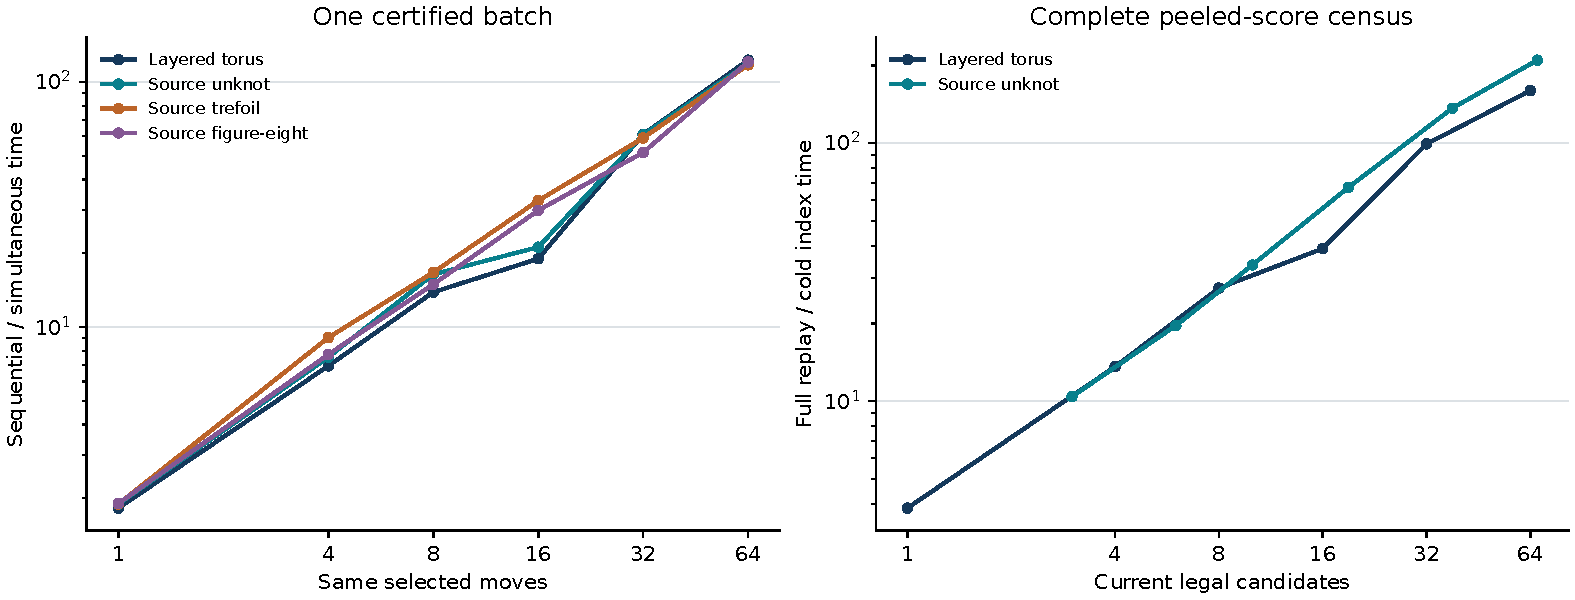
\includegraphics[width=\textwidth]{figures/geometric_performance.pdf}
\caption{Observed subroutine ratios, with three alternating paired rounds
per point. Left: simultaneous checked producer versus the existing literal
sequential composition on the same selected sites. Right: a freshly built
minima index and complete candidate census versus full individual geometric
replay of every candidate. Lines connect measured points; they are not
fitted asymptotic bounds.}
\label{fig:performance}
\end{figure}

\subsection{A cold index plus the entire peeled-score census}

This comparison starts the dynamic state from scratch on every timed run.
It includes the index construction and complete current candidate census.
The reference independently prepares the same input, performs every
candidate with the individual geometric producer and transport consumer,
and recomputes all vertex-link minima. The entire ordered list of site,
peeled Euler gain, and peeled piece saving agrees exactly. It is not a
comparison against a previously optimised static thirteen-prefix
implementation; the incoming report supplied a theorem for that pass,
not such an implementation.

\begin{table}[htbp]
\centering\small
\begin{tabular}{lrrrrrr}
\toprule
Family & Inserted sites & $t$ & Census $M$ & Full replay (s)& Cold index (s)& Ratio\\
\midrule
Layered &1&3&1&0.00135&0.00035&3.85\\
Layered &4&12&4&0.01738&0.00128&13.59\\
Layered &8&24&8&0.06480&0.00236&27.42\\
Layered &16&48&16&0.30292&0.00777&39.00\\
Layered &32&96&32&1.14917&0.01157&99.30\\
Layered &64&192&64&4.74531&0.02968&159.86\\
\midrule
Unknot &1&21&3&0.02030&0.00195&10.40\\
Unknot &4&24&6&0.04827&0.00246&19.62\\
Unknot &8&28&10&0.09583&0.00284&33.69\\
Unknot &16&76&19&0.50188&0.00745&67.37\\
Unknot &32&132&38&1.71692&0.01258&136.53\\
Unknot &64&204&67&5.09894&0.02432&209.69\\
\bottomrule
\end{tabular}
\caption{Complete peeled candidate scoring, including a fresh index on
the faster arm. The census can include legal sites beyond the inserted ones.}
\label{tab:peeling}
\end{table}

The tree-maintenance theorem concerns repeated local edits. These timings
test a more conservative cold-start query; they do not isolate an amortised
update speedup. A separate fresh-geometry audit checks 23 committed batches
and 45 moves across four families, including stable-vertex/fresh-root
bijections, link types, every triangle record, all thirteen-key prefixes,
and exact collective score agreement. All checks pass.

\subsection{The active-support lift reduces calls but loses elapsed time}

The active audit contains 20 partial-mask cases across seven genuine finite
triangulations. Seventeen have positive objective and compare complete
support discovery by efficient unary probes with the homogeneous lifted
query. The unary method skips coordinates whose activity is already
witnessed by an earlier LP point. This is therefore a meaningful small-LP
baseline, not an artificially padded fixed number of queries.

\begin{table}[htbp]
\centering\small
\begin{tabular}{lrrrrrr}
\toprule
Family & Masks & Unary calls & Lift calls & Unary (s) & Lift (s) & Lift/unary\\
\midrule
Fibonacci, $t=1$ &2&6&2&0.00177&0.01644&9.30\\
Fibonacci, $t=2$ &3&16&3&0.02559&0.21252&8.30\\
Fibonacci, $t=3$ &3&24&3&0.17221&1.22396&7.11\\
Fibonacci, $t=4$ &3&27&3&0.42699&4.12959&9.67\\
Branching torus, $t=5$ &3&31&3&0.68977&16.10012&23.34\\
Boundary attachment, $t=3$ &3&26&3&0.10197&1.14782&11.26\\
Finite trefoil, $t=5$ &3&3&0&0.22226&---&---\\
\bottomrule
\end{tabular}
\caption{Time sums across the specified masks. The last row terminates
after negative ordinary prechecks, so it does not run the lifted query.}
\label{tab:active-timing}
\end{table}

Across the 17 positive paired cases, the unary method uses 130 LP calls,
1,418 pivots, and 1.418307 seconds; the lift uses 17 calls, 1,449 pivots,
and 22.830456 seconds. The aggregate slowdown is 16.10-fold. The median
individual slowdown is 8.84-fold, the range is 5.89--38.48-fold, and the
lift wins no timing comparison. Similar pivot counts do not imply similar
work because the lifted tableau is much larger. These data support the
certificate interface but oppose enabling this dense implementation as a
general speed optimisation.

A separate exploratory direct lift of the unrestricted five-tetrahedron
trefoil root took 78.577357 seconds and 2,664 pivots to return nonpositive.
It is a single exploratory observation, not a repeated paired measurement.
The retained default audit uses a 25-second allowance per request and has
no cap outcomes. The ordinary precheck prevents this unnecessary lifted
query on the negative control.

\subsection{Complete search controls and independent replay}

\begin{table}[htbp]
\centering\small
\begin{tabular}{llrrrrr}
\toprule
Source & Precheck & Time (s) & Nodes & Branches & LP calls & Lifts\\
\midrule
Fibonacci 1 &yes&0.00105&3&0&3&0\\
Fibonacci 1 &no &0.04512&5&2&5&5\\
Fibonacci 2 &yes&0.17846&5&2&7&2\\
Fibonacci 2 &no &0.48030&6&3&6&6\\
Fibonacci 3 &yes&1.22946&6&3&9&3\\
Fibonacci 3 &no &3.29603&7&4&7&7\\
Finite trefoil &yes&2.45246&20&0&20&0\\
\bottomrule
\end{tabular}
\caption{Seven full anchored searches. The Fibonacci controls return
positive Euler; the finite trefoil proves no positive-Euler vector across
its 20 anchors. Every result has an independently replayed certificate.}
\label{tab:active-search}
\end{table}

The replay script checks 37 support certificates and all seven complete
normal-search certificates without importing an LP solver. Positive
meridian controls are additionally checked through the maintained
compressing-disc endpoint. The experimental active search does not include
the earlier mandatory-type propagation, so its branching on Fibonacci
inputs is not a measurement of the maintained recognizer's policy.
When no active query ran, an empty observed-rank statistic is not a proof
that the root rank is zero.

The final maintained-plus-overlay test run reports \fulltestcount{} tests
passing. It includes \focusedtestcount{} focused tests for the new
interfaces. Tests cover all 24 orders of four disjoint sites, all six
orders of three sites on each of three source exteriors, shared boundary
facets, true overlapping-star rejection, malformed/corrupted proofs,
producer-disabled consumer replay, exact large integer scales, callback
cancellation, and input immutability. Randomised algebraic audits compare
600 bounded matching instances with exhaustive search, including 300
small-cover cases with the general backend disabled. Three initial full-run
errors were missing historical fixture files; two byte-verified pinned
fixtures were restored, the affected tests passed, and the complete suite
was rerun. The retained logs distinguish that setup failure from the final
verified result.


\section{What these bounds do, and do not, imply asymptotically}
\label{sec:complexity}

\subsection{A complete collapse-only trajectory is a polynomial subroutine}

Let $V(t,B)$ bound the cost of the maintained finite-manifold and cocycle
preparations on $t$ tetrahedra with $B$-bit edge differences. Initial
height rows are assumed gauged, for example by subtracting their first
entry. If arbitrarily large common offsets are supplied, reading and
normalising those integers is charged separately in their actual input
bit length. We keep the preparation cost explicit. Let $\M(B)$ stand for a safe bound on the relevant exact
integer arithmetic cost; additions and comparisons are cheaper than general
multiplication. A complete current census has $O(t)$ candidates, because
there are at most $6t$ local edge occurrences. Sorting for greedy packing
costs $O(t\log(t+2))$ comparisons. The minima index and source-specific
matching add polynomial work independent of expanded surface weight.

\begin{proposition}[Cost and termination of the supplied local policy]
\label{prop:collapse-trajectory}
Start with a coherent cocycle on a valid triangulation with at most two
interior vertices. At each round, form the complete legal $3$--$2$ census,
choose a greedy maximal disjoint family, select its optimal peeled-Euler
subbatch with the minimum-omission rule, and commit it if nonempty. Stop
otherwise. Every committed round is nondecreasing in peeled Euler
characteristic; there are at most $t_0$ rounds and at most $t_0$ individual
collapses, where $t_0$ is the initial tetrahedron count. The maximum encoded
edge-difference bit length does not increase.

With polynomial $V$ and exact arithmetic, this is a polynomial subroutine
in $(t_0,B_0)$. A deliberately loose explicit bound is
\begin{equation}\label{eq:trajectory-cost}
 O\!\left(t_0 V(t_0,B_0)+
 t_0^2\log(t_0+2)\,\M(B_0+\log(t_0+2))\right),
\end{equation}
assuming a nondecreasing upper bound $V$. The lifetime maintenance work of
the corner index alone is only
$O(t_0\log(t_0+2))$ record operations.
\end{proposition}
\begin{proof}
The empty subbatch is available and has gain zero, so an optimum cannot
have negative gain. Every committed move reduces the number of tetrahedra
by one. Thus at most $t_0$ moves can be committed, and each nonempty round
contains at least one. The commuting theorem preserves the vertex types,
so the small-cover selection remains applicable. Every edge after a
$3$--$2$ move already occurred on the bipyramid boundary; its cocycle value
is unchanged. This proves the bit statement.

Charge each round its complete census, packing, reward computation,
linear small-cover matching, final emission, and constant number of
preparations. Bounding every current size by $t_0$ and the number of rounds
by $t_0$ gives \eqref{eq:trajectory-cost}. There are initially $4t_0$ corner
records; each collapse deletes twelve and inserts eight, so the total
number of index edits is $O(t_0)$. The balanced-tree theorem supplies the
last assertion.
\end{proof}

This proposition gives an honest finite local algorithm, including its
stopping condition. It makes no claim that the terminal coherent vector
contains a disc or that a stalled triangulation cannot be the unknot.
Repeating an uncontrolled $2$--$3$ repair phase is outside its proof.
Likewise, recording every endpoint of every round can still cost quadratic
space in $t_0$; the per-batch encoding theorem does not automatically supply
a linear-size transcript for an entire trajectory.

\subsection{A density hypothesis would give logarithmically many rounds}

\begin{corollary}[Conditional dense-census progress]
\label{cor:dense-progress}
Suppose a collapse-only trajectory as above has at least $\alpha t$
eligible distinct central edges whenever its current size is $t\ge40/\alpha$,
where $0<\alpha\le6$ is fixed. Then it reaches size below $40/\alpha$ in
$O(\alpha^{-1}\log(t_0+2))$ committed rounds.
\end{corollary}
\begin{proof}
The packed optimum retains at least
\[
 \lceil\alpha t/10\rceil-2\ge\alpha t/20
 \qquad(t\ge40/\alpha).
\]
Thus the next size is at most $(1-\alpha/20)t$. Repeated multiplication
proves the bound, using $-\log(1-\alpha/20)\ge\alpha/20$.
\end{proof}

The density assumption is not established for all diagram exteriors or
after arbitrary moves. A legal census can be sparse or empty. The corollary
is useful because it specifies an exact geometric statement that would
turn the batch-retention theorem into a round bound, without conflating
raw score, peeled score, and the number of removed tetrahedra.

\subsection{The normal-search ledger}

The active-face theorem isolates the factor
$\mathcal A(T)2^{\rho_{\max}}$. It supplies no universal reduction of this
factor. In fact, the unrestricted source lower bound rules out the proposal
that $\rho_{\max}$ is automatically polylogarithmic in crossing number.
The anchor count also needs separate attention. In a one-vertex finite
triangulation it is $4t$; in a triangulation with many vertices it is the
product of their corner degrees. The fact that there are only two
\emph{interior} vertices in the pulling source does not make that anchor
product small: the same source has $4n'$ boundary vertices. Confusing the
two vertex counts would erase a genuine source of combinatorial cost.

Complete-support certification, support minimisation of one admissible
point, and proving a small active ambiguity rank are three different
tasks. The first now has a compact interface. The second already has
classical LP-based solutions \cite{BurtonOzlen}. The third fails at the
unrestricted roots proved above. A promising parameter must therefore be
defined after stronger certified restrictions, or the algorithm must be
proved to reach an endpoint before traversing the large rank.

\subsection{A sufficient quasipolynomial contract}

For clarity, consider a future complete architecture with at most $R(n)$
outer stages. At each stage suppose it covers all required geometric
choices by a tree of depth $h(n)$, branching at most $(ct(n)+c)^d$ ways per
node for fixed positive constants $c,d$, and each node performs at most $A(n)$ normal queries with active
rank at most $\rho(n)$. Suppose all state sizes are bounded by $t(n)$ and
all arithmetic inputs by $B(n)$ bits, with polynomial local producers and
consumers. A sufficient upper bound is
\begin{equation}\label{eq:qp-ledger}
 R(n) A(n) 2^{\rho(n)}
 (ct(n)+c)^{O(h(n))}\poly(t(n),B(n)).
\end{equation}
For example, if $t,B,R$ are polynomial in $n$,
$\log A(n)=O((\log n)^a)$, $\rho(n)=O((\log n)^b)$, and
$h(n)=O((\log n)^c)$ for fixed exponents, then
\eqref{eq:qp-ledger} is
\[
 \exp\!\left(O((\log n)^{\max\{1,a,b,c+1\}})\right).
\]
This is an elementary composition bound, not a theorem that those
hypotheses hold. It displays the obligations a genuine quasipolynomial
proof must discharge.

The present results improve the local polynomial factor and eliminate
$2^{|E|}$ subbatch enumeration for a fixed disjoint family. They do not
prove geometric witness coverage, the depth bound $h$, the restricted-rank
bound $\rho$, or the anchor bound $A$. The explicit root obstruction also
shows why replacing the last two obligations by an empirical observation
would not suffice. Classical compressed component algorithms avoid
dependence linear in expanded normal weight \cite{AHT}; they do not bound
the number of global choices by themselves.


\section{Further research: statements worth proving next}
\label{sec:research}

The following questions are ordered by how directly a positive answer
would improve the current algorithm. Each separates a mathematical target
from an implementation experiment. Several may have negative answers;
explicit counterfamilies would still prevent investment in an invalid
complexity strategy.

\subsection{Geometric progress and the correct search space}

\paragraph{1. When must a useful collapse exist?}
Characterise coherent primitive-meridian fibres for which a legal $3$--$2$
move or nonempty optimum packed subbatch exists before an essential disc
is exposed. A strong target is a density or amortised density theorem of
the form in \cref{cor:dense-progress}. A weaker useful target is a bounded
repair lemma: a stalled state admits at most $f(t)$ certified expansions
followed by a batch that reduces a well-founded, explicitly encoded
potential. Experiments should record empty censuses, small censuses,
negative singleton scores, and stalls separately, because the matching
theorem resolves only collective selection once candidates exist.

\paragraph{2. Can the two-pole structure survive more powerful reductions?}
The current fast selector survives vertex-preserving $2$--$3$ and $3$--$2$
moves. Crushing, collapsing boundary cells, idealisation, and handle
normalisation can alter the vertex links or the representation. Prove an
interface theorem retaining a bounded set of interior reward vertices,
or identify an equally small parameter in the new representation. A finite
two-pole triangulation and an ideal triangulation have different local
link contracts; transferring formulas between them requires a proof.

\paragraph{3. Optimise the disjoint ground family, not only its subbatches.}
The degree-nine argument gives a constant-factor cardinality packing, and
the new matching theorem exactly solves selection inside that packing.
It leaves the choice among overlapping regions unresolved. Determine
whether conflict graphs arising from legal bipyramids have additional
structure beyond bounded degree that permits an exact or suitably
certified approximation algorithm for the final peeled objective.
An arbitrary bounded-degree graph does not acquire easy maximum-weight
independent-set optimisation merely from its degree bound. Small geometric
instances should compare every packing, every subbatch, and greedy
packing followed by matching to identify the actual lost opportunity.

\paragraph{4. Is peeled Euler characteristic the right policy potential?}
The shared-vertex counterexample proves a failure of additivity on a genuine
solid torus, but its supplied cocycle is exact. Investigate the same
interaction under primitive meridional cohomology and boundary constraints.
More broadly, seek a potential that combines tetrahedron count, peeled
Euler characteristic, essential-boundary information, and compressed
component structure. Its monotonicity must survive globally identified
vertices and sphere components. A scalar score that increases while
losing the relevant disc component would not establish witness coverage.

\paragraph{5. Bound the number of genuinely different geometric choices.}
Commutation identifies all orders of one fixed set of disjoint moves.
It does not identify different sets or repairs through overlapping sites.
Develop a canonical transition certificate, a confluence theorem on a
restricted class, or a partial-order reduction that preserves at least
one successful witness path. The target is a bound on distinct relevant
states, with a proof that the quotient preserves the topological endpoint,
rather than a reduction in the number of syntactic transcripts alone.

\subsection{Admissibility, support, and certificate-efficient LP}

\paragraph{6. Remove the explicit root obstruction only with a sound quotient.}
The local directions $w_a$ change all three quadrilaterals together and are
invisible to face-arc matching. Can one quotient or eliminate those
directions while preserving admissible positive-Euler existence, including
the triangle anchors and Euler objective? Their compatibility effect is
nonlinear, so simply deleting them from a rank computation is unsound.
A useful answer would give a reconstruction theorem from a quotient
solution and a polynomial certificate of every excluded alternative.
Alternatively, prove that a natural strengthened relaxation still has a
linear ambiguity family; that would rule out another tempting route.

\paragraph{7. Relate active rank to mandatory propagation after restrictions.}
The incoming Fibonacci result has zero mandatory guess budget, while the
unrestricted active rank here is linear. These parameters measure different
things. Define a parameter for a \emph{certified adaptive trajectory} after
all currently forced types have been propagated, and ask whether it is
polylogarithmic on a topologically meaningful class. The quantifiers matter:
the existence of one easy witness is weaker than a complete negative
decision procedure. Any bound must include the dual certificates and
incompatible branches needed to prove absence.

\paragraph{8. Produce the active-support certificate more cheaply.}
The current homogeneous lift adds $O(N+m)$ auxiliary structure to an already
degenerate LP and is slower in the retained audit. Investigate sparse
relative-interior methods, a reused primal/dual basis, incremental forced
zero aggregation, or a hybrid that invokes the full lift only after a
measured trigger. Basis reuse itself has established normal-surface
precedents \cite{BurtonTree}; novelty should be measured by the resulting
certificate size or verified work reduction. Benchmark rational bit growth,
pivots, matrix density, calls, producer time, and replay time together.

\paragraph{9. Compress anchor coverage.}
Find a polynomial or quasipolynomial certificate representing the complete
union of vertex-anchor cones without listing every anchor tuple. Shared
subproofs, symmetry, vertex-link quotient coordinates, or a proof-producing
elimination rule may help. A checker must reconstruct why every canonical
normal vector is covered; a cache containing only visited anchors is not a
negative certificate. The two-pole source is a useful test because it has
few interior vertices but linearly many boundary vertices.

\subsection{Compressed topology and a global complexity theorem}

\paragraph{10. Make hierarchy transitions preserve all required markings.}
Relate the repository's compressed normal components and boundary moments
to the boundary patterns and parallelity data needed by hierarchy methods.
Specify what a transition certificate records, how it is independently
verified, and how its encoded size changes. The 2026 hierarchy work offers
concrete topological progress measures \cite{Lackenby2026}, but importing
one of them requires a proved correspondence with this triangulation and
cocycle implementation. Boundary curve normalisation must count every
parameter required by its algorithm; the simplification parameter in the
current fast-curve theorem cannot be suppressed \cite{LackenbyCurves}.

\paragraph{11. Prove a bit-size invariant through repairs and regauging.}
Collapse-only transport has a nonincreasing edge-difference bound. Global
regauging, LP extraction, expansions, and hierarchy repairs need a joint
bound on integer and rational sizes. Establish a potential measuring
encoding length as well as topological complexity. An algorithm may take
few combinatorial steps but still create excessively large coordinates;
counting arithmetic operations alone would miss that growth.

\paragraph{12. Export matching and transition optimality certificates.}
The general matching backend currently supplies a checked attained value
without exporting an Edmonds dual. Add a producer for a sparse dual,
including the integer scaling for minimum omissions, and verify it through
the existing independent interface. For the two-cover case, a small
certificate of the per-pole best endpoint choices should suffice. This is
primarily a trust-boundary improvement; move correctness already has an
independent geometric consumer.

\paragraph{13. Test whole-policy effects on source-bound hard families.}
The retained timing work fixes the same moves or the same candidate queries
on both sides. The next experiment should compare complete policies with
identical source diagrams, endpoint checks, and resource accounting. Include
hard unknots, nontrivial knots escaping early filters, repeated expansions,
and low-density stalls. Report failed budgets and regressions, not only
successful reductions. Separate time to find a witness, certificate size,
and independent replay time. No finite corpus alone supplies a worst-case
theorem, but it can identify which missing lemma would have practical value.

\paragraph{14. Close the cost ledger with explicit quantifiers.}
The eventual target is a theorem covering every input diagram and every
state required by a complete search, with bounded transition depth,
branching, anchors, and bit sizes as in \eqref{eq:qp-ledger}. A resource-limited
research module that returns an inconclusive status is useful engineering;
it is not a total quasipolynomial decision algorithm. The most productive
next theorem would bound a presently uncontrolled factor on a nontrivial,
source-defined class and provide the certificate that makes that bound
usable by the implementation.


\appendix
\section{Package map and reproduction}
\label{sec:reproduction}

The archive is rooted at
\texttt{unknot\_active\_faces\_batched\_descent\_20261009/}.
The top-level README gives exact commands and the integration contract.
The manifest records source revisions, incoming dependency hashes, and
the identities of retained fixtures. Relative paths are used throughout
the executable research scripts.

\begin{longtable}{p{0.30\textwidth}p{0.63\textwidth}}
\toprule
Path & Contents \\
\midrule
\endhead
\texttt{article/} & Complete modular \LaTeX{} source, final PDF, and vector
performance figure. \\
\texttt{code/fast/} & Pinned supporting implementation, additive modules,
focused and maintained tests, benchmark and replay scripts. \\
\texttt{code/synthesis/data/} & The two pinned historical fixtures needed
by maintained test imports. \\
\texttt{code/reports/} & Historical oracle helpers required by existing
tests, with provenance recorded. \\
\texttt{integration/} & Additive patch against the pinned tree, file
lineage, and the patch-check result. \\
\texttt{evidence/geometry/} & All 24 fixed-batch inputs, source bindings,
expansion records, both witnesses, and raw paired timing samples. \\
\texttt{evidence/counterexample/} & The realized shared-vertex example,
portable construction, retained 24-tetrahedron seed, and batch witness. \\
\texttt{evidence/validation/} & Complete test logs, independent dynamic
audit, cold-census timings, environment, and replay summaries. \\
\texttt{tools/} & Figure regeneration and package verification helpers. \\
\bottomrule
\end{longtable}

From \texttt{code/fast/}, the fast certificate checks do not need an LP
solver or optional graph library:
\begin{lstlisting}
python -S active_research/replay.py
python -S batched_descent_research/replay_evidence.py
\end{lstlisting}
The full test suite is run with:
\begin{lstlisting}
python -m unittest discover -s tests -v
\end{lstlisting}
NetworkX enables the five general matching tests; the source-specific
small-cover tests still run with site packages disabled. Exact geometric
and arithmetic replay use only included modules. The optional regeneration
of the barycentric torus from its original triangulation library is
separate from replay of the retained seed.

The checked producer benchmark can be rerun with the supplied
\path{batched_descent_research/benchmark_batch.py}; it reconstructs
source-bound inputs and performs alternating paired runs. Its command-line
help describes size and output controls. The peeled-census benchmark takes
the retained evidence directory as an explicit argument, and
\texttt{active\_research/benchmark.py} reconstructs its masks and support
queries from the supplied source file. Reproducing exact elapsed times is
not expected across hosts; reproducing exact face pairings, heights,
supports, objective values, and valid certificates is the relevant
correctness condition.

Compile the article from its directory with:
\begin{lstlisting}
latexmk -pdf -interaction=nonstopmode -halt-on-error article.tex
\end{lstlisting}
The final PDF was rendered and visually checked in addition to successful
\LaTeX{} compilation. The package does not require downloading the three
large incoming archives: the few unchanged prerequisite modules are
included and explicitly attributed. It also does not include a new claim
that the complete recognizer has quasipolynomial worst-case complexity.

\section{The general two-endpoint algebraic extension}
\label{sec:general-reward-extension}

The exported algebraic selector allows nonnegative costs $r_i$ and at most
two nonnegative endpoint rewards $c_{vi}$ even when the geometric bound
$c_{vi}\le r_i$ is absent. This extension is not needed for the main
geometric theorem. Here is the correctness argument for its implementation.
Let
\[
 b_v=\max\bigl(0,\max_i(c_{vi}-r_i)\bigr).
\]
A two-endpoint item $i$ on distinct vertices $u,v$ receives adjusted edge
weight $c_{ui}+c_{vi}-r_i-b_u-b_v$. Discard nonpositive edges and retain the
largest parallel edge. Then the optimum of $H$ is the sum of the $b_v$
plus the maximum adjusted matching weight.

To prove the upper bound, take any omitted set and assign each vertex's
positive maximum reward to one attaining item. Delete items assigned no
vertex; their costs are nonnegative. Each remaining item is assigned one
or two vertices. A singly assigned item contributes at most $b_v$. The
doubly assigned items form a matching on their assigned pairs and
contribute their adjusted weights plus those vertices' baselines. Unused
nonnegative baselines can only enlarge the bound. Dropping nonpositive
adjusted edges can also only enlarge it.

For the reverse bound, choose a maximum adjusted matching and, for each
unmatched vertex with positive baseline, choose a baseline-attaining item.
Take the union of these items with the matching items. At each vertex
the actual maximum reward is at least the assigned one; an item chosen
more than once is paid for only once, so its actual total cost is at most
the sum charged in the assignment. Thus $H$ is at least the proposed
matching-plus-baseline value. The upper bound proves equality. In the
geometric case all baselines vanish, and this reduces to the main theorem.
Outside that case the secondary matching-cardinality rule need not minimise
the number of reconstructed singleton items; the API records this limit.


\clearpage
\begin{thebibliography}{99}
\small\raggedright
\setlength{\itemsep}{1.5pt}
\setlength{\parsep}{0pt}
\setlength{\parskip}{0pt}
\addcontentsline{toc}{section}{References}

\bibitem{ProveItSource}
Vladimir Reshetnikov, \emph{ProveIt: Topology/UnknotRecognition}, repository
revision \basecommit. In particular,
\texttt{synthesis/diagram\_exterior.tex} and the maintained
\texttt{fast/fastunknot/diagram\_exterior.py} source construction.
\url{https://github.com/VladimirReshetnikov/ProveIt/tree/66098968e88bba797143ac1bf7ad0ac4c5f697df/Topology/UnknotRecognition}.

\bibitem{priorDual}
ProveIt research continuation, \emph{Dual Certificates and Forced Quadrilateral Propagation for Unknot Recognition},
9 October 2026. Incoming archive
\texttt{unknot\_dual\_certificates\_20261009.zip}; Git blob
\texttt{1e0764557877847c2d8df1e96256b82795505b81}.
Available in the pinned repository's \texttt{docs/incoming/} directory.

\bibitem{priorSupport}
ProveIt research continuation, \emph{Support-Sensitive Certificates for
Unknot Recognition: Optimal coordinate transport, component profiles,
and linear unit-pivot ray certificates}, 9 October 2026. Incoming archive
\texttt{unknot\_support\_sensitive\_certificates\_20261009.zip}; Git blob
\texttt{afdf1aa14f39ba54538f6e72f0c2cc4e4c4b3ce5}.

\bibitem{priorTransport}
ProveIt research continuation, \emph{Cocycle Transport and Ordered Boundary Interfaces for Unknot Recognition},
9 October 2026. Incoming archive
\texttt{unknot\_geometric\_transport\_20261009.zip}; Git blob
\texttt{c86bb8cfb5142abe2a7732a2f078ac1dde3cb00d}.

\bibitem{GoldmanTucker}
A. J. Goldman and A. W. Tucker, Theory of linear programming,
in H. W. Kuhn and A. W. Tucker (eds.), \emph{Linear Inequalities and
Related Systems}, Annals of Mathematics Studies 38, Princeton University
Press, 1956.

\bibitem{Edmonds1965}
Jack Edmonds, Maximum matching and a polyhedron with 0,1-vertices,
\emph{Journal of Research of the National Bureau of Standards B}
69B (1965), 125--130.
\url{https://nvlpubs.nist.gov/nistpubs/jres/69B/jresv69Bn1-2p125_A1b.pdf}.

\bibitem{NetworkX}
NetworkX developers, \texttt{max\_weight\_matching}, version 3.7
documentation, accessed 9 October 2026.
\url{https://networkx.org/documentation/stable/reference/algorithms/generated/networkx.algorithms.matching.max_weight_matching.html}.

\bibitem{BurtonOzlen}
Benjamin A. Burton and Melih Ozlen, \emph{A fast branching algorithm for
unknot recognition with experimental polynomial-time behaviour},
arXiv:1211.1079v3, 2014. See Lemmas 7--8, Algorithm 9, and Theorem 12.
\url{https://arxiv.org/abs/1211.1079}.

\bibitem{BurtonFaces}
Benjamin A. Burton, Maximal admissible faces and asymptotic bounds for
the normal surface solution space, \emph{Journal of Combinatorial Theory,
Series A} 118 (2011), 1410--1435.
\url{https://arxiv.org/abs/1004.2605}.

\bibitem{BurtonTree}
Benjamin A. Burton and Melih Ozlen, \emph{A tree traversal algorithm for
decision problems in knot theory and 3-manifold topology},
arXiv:1010.6200. See the incremental LP routines in Section 3 and the
arithmetic bounds in Section 4.
\url{https://arxiv.org/abs/1010.6200}.

\bibitem{AHT}
Ian Agol, Joel Hass, and William Thurston, The computational complexity
of knot genus and spanning area, \emph{Transactions of the American
Mathematical Society} 358 (2006), 3821--3850.
\url{https://arxiv.org/abs/math/0205057}.

\bibitem{LackenbyTalk}
Marc Lackenby, \emph{Unknot recognition in quasi-polynomial time},
Oxford technical talk handout, March 2021, 34 pages.
The explicit running-time expression in the technical handout is
$2^{O((\log n)^3)}$.
\url{https://people.maths.ox.ac.uk/lackenby/quasipolynomial-talk-oxford-compressed.pdf}.

\bibitem{Lackenby2026}
Marc Lackenby, \emph{Incompressible surfaces, hierarchies and unknot
recognition}, arXiv:2607.23350v1, 25 July 2026, 54 pages.
\url{https://arxiv.org/html/2607.23350v1}.

\bibitem{LackenbyCurves}
Marc Lackenby, Some fast algorithms for curves in surfaces,
\emph{Discrete \& Computational Geometry} (2026),
doi:10.1007/s00454-026-00845-7. Author manuscript:
\url{https://people.maths.ox.ac.uk/lackenby/AlgorithmsSurfaces13jan26.pdf}.

\end{thebibliography}


\end{document}
